% =============================================================================
% When the Stars Disagree
% arXiv preprint — pdflatex + CJKutf8, two-column
% =============================================================================
\documentclass[10pt,a4paper]{article}

% --- Packages ----------------------------------------------------------------
\usepackage[utf8]{inputenc}
\usepackage[T1]{fontenc}
\usepackage{CJKutf8}
\usepackage{amsmath,amssymb,amsfonts}
\usepackage{booktabs}
\usepackage{multirow}
\usepackage{graphicx}
\usepackage{xcolor}
\usepackage{hyperref}
\usepackage[margin=0.75in]{geometry}
\usepackage{enumitem}
\usepackage{float}
\usepackage{caption}
\usepackage{subcaption}
\usepackage{siunitx}
\usepackage{longtable}
\usepackage[numbers,sort&compress]{natbib}
\usepackage{xurl}  % Better URL line-breaking than url
\usepackage{authblk}
\usepackage{pgfplots}
\usepackage{tikz}
\usepackage{gensymb}
\usepackage{adjustbox}
\usepackage[framemethod=tikz]{mdframed}

\pgfplotsset{compat=1.18}
\usepgfplotslibrary{statistics}

\setlength{\columnsep}{18pt}

\hypersetup{
    colorlinks=true,
    linkcolor=blue!70!black,
    citecolor=green!50!black,
    urlcolor=blue!60!black,
}

% CJK helper
\newcommand{\zh}[1]{\begin{CJK}{UTF8}{bsmi}#1\end{CJK}}

% ORCID helper
\newcommand{\orcidlink}[1]{%
  \href{https://orcid.org/#1}{\textcolor{green!50!black}{\textsf{iD}}}%
}

% pgfplots color scheme
\definecolor{sbblue}{HTML}{2166AC}
\definecolor{sxorange}{HTML}{D6604D}
\definecolor{jplgray}{HTML}{636363}
\definecolor{de441blue}{HTML}{4393C3}
\definecolor{de405red}{HTML}{B2182B}

% --- Title -------------------------------------------------------------------

\title{%
  \textbf{When the Stars Disagree:}\\[4pt]
  \large A Cross-Civilizational Analysis of Computational Errors\\
  in Astronomical Divination%
}

\author[1]{Albert Kwun Tai Hui\,\orcidlink{0009-0000-8978-0231}}
\affil[1]{Security Ronin}

\date{March 2026}

% =============================================================================
\begin{document}

\twocolumn[
\maketitle

\begin{abstract}
\noindent
Astronomical divination systems---from Chinese \zh{四柱八字}
and Indian Jyotish to Western horoscopic astrology---depend on
precise ephemeris computation, yet the software that serves hundreds
of millions of practitioners routinely produces discordant results.
This paper does not evaluate whether any divination system yields
valid predictions; it analyzes whether the underlying astronomical
computations are \emph{correct}.

We identify and quantify seven categories of computational error
in widely-used software for five Chinese systems (\zh{八字},
\zh{奇門遁甲}, \zh{紫微斗數}, \zh{大六壬}, \zh{七政四餘}), ranging
from daylight saving time mishandling and true solar time neglect
to ephemeris truncation and historical $\Delta T$ uncertainty.  A
three-way statistical validation against \zh{壽星萬年曆} (sxwnl)
and JPL~DE441 across 2,284~years demonstrates mean solar term
timing accuracy of $1.05$~seconds ($N = 1{,}008$, max $= 3.05$~s).

Three cross-cutting reference-frame problems recur across
civilizations: the choice of prime meridian (Chinese \zh{天下之中},
Indian Ujjain, Ptolemy's Fortunate Islands, Greenwich), the
tropical-sidereal zodiac divergence ($\sim 24\degree$ by 2026),
and the birth-time recording precision floor.  These are not
uniquely Chinese difficulties but universal features of
coordinate-dependent astronomical traditions.  We further analyze
the methodological challenges of heuristic validation, the
shared-chart (\zh{共盤問題}) statistical problem, and the
degrees-of-freedom critique applicable to interpretive
frameworks.  The five Chinese systems form a computational
robustness spectrum from astronomically fragile (\zh{七政四餘})
to maximally robust (\zh{紫微斗數}), reflecting deliberate
architectural trade-offs between celestial fidelity and
computational permanence.
\end{abstract}

\medskip
\noindent\textbf{Keywords:} computational astronomy, astronomical
divination, Chinese calendar, BaZi, Jyotish, solar terms, lunar
phases, planetary ephemeris, VSOP87, JPL DE441, $\Delta T$,
intercalation, true solar time, prime meridian, tropical zodiac,
sidereal zodiac, ayanamsa, reference frame, statistical validation,
error analysis

\vspace{1em}
]

\footnotetext[0]{Preprint. \texttt{arXiv:2603.xxxxx [astro-ph.IM]}}


% =============================================================================
\section{Introduction}
\label{sec:intro}

\begin{mdframed}[
  linecolor=black!40,
  backgroundcolor=black!3,
  roundcorner=4pt,
  linewidth=0.5pt,
  innertopmargin=8pt,
  innerbottommargin=8pt,
]
\small\noindent\textbf{A note on scope and intent.}
The author holds no position on whether astronomical divination
systems produce valid predictions about human affairs.  The claim
that celestial configurations at birth reflect or influence a
person's life trajectory involves metaphysical commitments that
lie outside the scope of empirical investigation as normally
understood.

The present investigation originated in skepticism.  An examination
of the computational models underlying several Chinese metaphysical
software applications revealed that many implementations contained
astronomical drift, timezone errors, and calendar miscomputations
by modern standards---errors that their users had no means to detect.
The gap between the precision these systems \emph{claim} and the
precision their software \emph{achieves} was large enough to
warrant systematic investigation.  That investigation---initially
motivated by the question ``are these apps even computing the
astronomy correctly?''---expanded into the cross-civilizational
error analysis presented here.

This paper analyzes whether the astronomical computations are
\emph{correct on their own terms}: whether the Sun's ecliptic
longitude, the lunar phase, or the planetary position is computed
accurately.  A horoscope derived from a wrong planetary position
is wrong even by its own logic, regardless of whether horoscopes
have any merit.  The distinction between computational correctness
and interpretive validity is fundamental throughout.
\end{mdframed}

\medskip

Astronomical divination---the practice of deriving meaning from
celestial configurations at the moment of birth, decision, or
event---has arisen independently across civilizations.  Chinese
\zh{四柱八字}, Indian Jyotish, Western horoscopic astrology, and
Mesoamerican calendar systems all share a common computational
dependency: the accurate determination of celestial positions at a
specific moment in time.  The astronomical techniques differ (solar
terms, lunar mansions, zodiacal signs, Long Count cycles), but the
underlying requirement is identical: precise ephemeris computation.

This paper examines five Chinese systems that span the full range of
astronomical dependency---from purely solar (\zh{八字}) through
solar-lunar (\zh{紫微斗數}, \zh{大六壬}) to fully planetary
(\zh{七政四餘})---and demonstrates that the computational errors
affecting them are not uniquely Chinese but recur wherever
coordinate-dependent astronomy meets traditional practice.  The same
reference-meridian problem that shifts a Chinese \zh{時辰} boundary
shifts an Indian \textit{lagna} (Ascendant); the same
tropical-sidereal divergence that confounds Chinese 28-mansion
placements confounds Indian \textit{rashi} assignments.

The Chinese calendrical system (\zh{曆法}) is one of humanity's oldest
continuous astronomical traditions, with systematic records spanning over
2,700~years \cite{stephenson2016}. At its computational core lies the
determination of two celestial cycles: the Sun's ecliptic longitude,
defining the 24 solar terms (\zh{二十四節氣}), and the Moon's phases,
defining the lunar months.  Since 2016, UNESCO has recognized the 24 solar
terms as part of humanity's Intangible Cultural Heritage \cite{unesco2016}.

This paper makes five contributions:
\begin{enumerate}[label=(\roman*)]
  \item An analysis of how five Chinese metaphysical systems depend on
        the solar-lunar-planetary computational pipeline, forming a
        robustness spectrum from astronomically fragile to maximally
        robust (Section~\ref{sec:systems});
  \item A taxonomy of computational errors---from daylight saving time
        mishandling to ephemeris truncation---organized by accessibility
        from practical to technical
        (Section~\ref{sec:errors});
  \item A cross-civilizational analysis of reference-frame problems
        (meridians, tropical vs.\ sidereal zodiac, time regimes) showing
        these are universal, not culture-specific
        (Section~\ref{sec:meridians});
  \item A three-way statistical validation demonstrating sub-second solar
        term accuracy across 2,284~years (Section~\ref{sec:validation});
  \item A methodological critique of heuristic validation, the
        shared-chart statistical problem, and degrees-of-freedom
        over-fitting in interpretive frameworks.
\end{enumerate}


% =============================================================================
\section{The Five Systems and Their Astronomical Dependencies}
\label{sec:systems}

The five systems form a spectrum from purely solar to fully planetary,
unified by their shared dependency on precise astronomical computation.
The first four---\zh{八字}, \zh{奇門遁甲}, \zh{紫微斗數}, and
\zh{大六壬}---use abstract stem-branch cycles anchored to solar and lunar
events. The fifth, \zh{七政四餘}, uses \emph{real} planetary positions,
making it the culmination of the accuracy argument.

\subsection{\zh{八字}: Solar Foundation}

\zh{八字}~\cite{wikipedia_fourpillars} is computationally grounded in
the 24 solar terms (\zh{二十四節氣}), which the tradition interprets
through the theoretical framework of \zh{氣} (qi)---a concept of
seasonal cyclicity driven by the Sun's annual motion.  The
correspondence between the five elements (\zh{五行}) and the
seasons---\zh{寒} (cold/winter), \zh{濕} (damp/late summer), \zh{暑}
(heat/summer), \zh{熱} (warmth/early summer)---reflects the
observable astronomical cycle of solar declination, which the system
maps onto a framework for analyzing human affairs.  Regardless of
whether this mapping has any validity, the computational pipeline is
entirely \emph{solar}: VSOP87D $\to$ apparent longitude $\to$ solar
term crossing $\to$ pillar assignment.

\subsection{\zh{奇門遁甲}: The 360-Day Problem}
\label{subsec:qimen}

\zh{奇門遁甲} (\textit{Q\'{i} M\'{e}n D\`{u}n Ji\v{a}}, ``Strange Gates,
Hidden Stems'') is one of the Three Arts (\zh{三式}) of Chinese divination,
alongside \zh{太乙神數} and \zh{六壬}. Its computational framework layers
six interacting systems---the Nine Palaces (\zh{九宮}), Eight Gates
(\zh{八門}), Nine Stars (\zh{九星}), Eight Spirits (\zh{八神}), Heavenly
Stems (\zh{天干}), and Earthly Branches (\zh{地支})---onto a temporal
grid of 1,080 unique configurations called \zh{局}
(formations)\footnote{The number derives from
$3 \text{ \zh{元}} \times 6 \text{ formations} \times 2 \text{ (\zh{陽遁}/\zh{陰遁})} \times 9 \text{ palaces} = 1{,}080$
in the standard \zh{陽遁}/\zh{陰遁} system.}.

Each \zh{局} is determined by the relationship between the current moment
and the surrounding solar terms. Time is divided into \zh{元} (epochs):
each solar term (\zh{節}) governs three \zh{元} (upper, middle, lower),
and each \zh{元} spans five days. Since there are 24 solar terms,
the theoretical year is $24 \times 3 \times 5 = 360$ days.

The fundamental computational problem is that the actual tropical year is
365.2422 days---a surplus of $\sim$5.25 days per year. This progressive
misalignment between the sexagenary cycle and actual solar term boundaries
is called \zh{超神} (``surpassing the spirits''). When a solar term arrives
and ``catches up'' with the cycle, it is called \zh{接氣} (``receiving the
qi''). Three competing methods have emerged to handle this discrepancy.

\subsubsection{\zh{置閏法} (Intercalation---the Ancient Method)}

The oldest method, encoded in the canonical \zh{煙波釣叟賦}
(\textit{Rhapsody of the Smoky-Wave Fishing Elder}) \cite{yanbo_diaosou}, strictly follows the
sexagenary cycle. When the \zh{超神} gap between the cycle marker
(\zh{符頭}) and the actual solar term exceeds 9 days, an intercalary period
(\zh{閏局}) is inserted. Critically, intercalation occurs only at
\zh{芒種} and \zh{大雪}---the solar terms immediately preceding the
solstices---effectively doubling those terms from 15 to 30 days.

This method treats the sexagenary cycle as primary and astronomical reality
as secondary. Its advantage is mathematical regularity; its disadvantage is
that the \zh{閏局} period is governed by a formation that no longer reflects
the prevailing seasonal \zh{氣}.

\subsubsection{\zh{拆補法} (Splitting---the Song Dynasty Reform)}

First documented in \zh{遁甲符應經} \cite{dunjia_fuying} (Jingyou era, 1034--1038~CE), this
method treats the solar term boundary as primary. When a \zh{節} arrives
mid-cycle, the current five-day period is \emph{split} at the exact solar
term moment:

\begin{itemize}
  \item Days before the \zh{節}: continue using the previous \zh{局}.
  \item Days after the \zh{節}: begin the new \zh{局} sequence.
  \item The proportional split within the transitional day requires knowing
        the solar term time to sub-hour precision.
\end{itemize}

This method, championed by modern practitioners such as Zhang Zhichun
(\zh{張志春})~\cite{zhang_zhichun}, produces a smooth transition aligned with seasonal reality
but sacrifices the mathematical elegance of the sexagenary cycle. It is the
dominant method in contemporary practice.

\subsubsection{\zh{茅山法} (Maoshan---the Daoist Alternative)}

A third method, developed by Maoshan Daoists during the Yuan--Ming
period\footnote{This dating is traditional attribution; the
\zh{茅山法}'s exact origin is poorly documented and no surviving
Yuan--Ming text provides a definitive provenance.},
starts the upper \zh{元} at the exact solar term moment and runs each
\zh{元} for exactly 60 \zh{時辰} ($= 5$ days), regardless of Branch
associations. This eliminates both the intercalation problem and the
splitting problem but breaks the traditional correspondence between
\zh{元} and specific sexagenary day-groups.

\subsubsection{Computational Precision Requirements}

The ``danger zone'' near solar term boundaries spans approximately
$\pm 2$ hours (one \zh{時辰}). Under the \zh{拆補法}, any divination
moment falling within this window requires sub-hour solar term precision to
determine which \zh{局} applies. Approximately 1.1\% of randomly-chosen
moments fall near a boundary\footnote{Each solar term boundary has a
$\pm 2$-hour danger zone (4~hours total). With 24~boundaries per year:
$24 \times 4 = 96$~hours out of $365.25 \times 24 = 8{,}766$~hours,
yielding $96 / 8{,}766 \approx 1.1\%$. While this percentage is small,
the consequences of a wrong \zh{局} assignment are total---the entire
divination board changes.}.

The validation in Section~\ref{sec:validation} demonstrates 1--3\,s solar
term accuracy, resolving the \zh{拆補法} split to within
$\sim 1 / 86{,}400 \approx 0.001\%$ of a day---effectively eliminating
astronomical computation as a source of \zh{局} assignment error.

The debate between methods has persisted since the Song dynasty and reflects
a fundamental tension between mathematical regularity (the sexagenary cycle)
and observational astronomy (the solar terms). It is structurally analogous
to the lunar calendar's \zh{閏月} mechanism
(Section~\ref{subsec:error_2033}): both are intercalation strategies that
reconcile incommensurate cycles.

\subsection{\zh{紫微斗數}: The Lunar Calendar Dependency}
\label{subsec:ziwei}

\zh{紫微斗數} (\textit{Z\v{i} W\={e}i D\`{o}u Sh\`{u}}, ``Purple Star
Calculation'') is a Chinese divination system attributed to the Daoist
sage Chen Tuan (\zh{陳摶}, also known as \zh{陳希夷}, c.~871--989~CE) and
later codified in two Ming-dynasty texts: the \zh{紫微斗數全書}
(\textit{Complete Book}, attributed to Luo Hongxian \zh{羅洪先}) \cite{zwds_quanshu} and the
\zh{紫微斗數全集} (\textit{Complete Collection}) \cite{zwds_quanji}.

Unlike \zh{八字}, which maps birth time directly to solar term boundaries,
\zh{紫微斗數} constructs a 12-palace fate chart (\zh{命盤}) from the
\emph{lunar} calendar date. The system distributes 14 major stars---led by
\zh{紫微} (Purple Star/Polaris) and \zh{天府} (Celestial Treasury)---across
12 life palaces (\zh{命宮}, \zh{兄弟宮}, \zh{夫妻宮}, etc.) using purely
algorithmic formulas. These are ``virtual'' stars: their positions are
computed from calendar arithmetic, not from actual astronomical
observations.

\subsubsection{The Computational Chain}

The chart construction depends on four lunar-calendar inputs: year, month, day, and
hour. The lunar month is the most consequential: changing it by even one
shifts the \zh{命宮} (Life Palace), the \zh{五行局} (Five-Element
Configuration), and consequently the positions of all 14 major stars. The
computational dependency chain is:

\begin{enumerate}
  \item \textbf{New moon timing} (\zh{合朔}): Each lunar month begins at
        the astronomical conjunction. Computing the exact new moon requires
        a lunar ephemeris (e.g., ELP/MPP02 \cite{ytliu_sunmoon}).
  \item \textbf{Intercalary month determination} (\zh{閏月}): The standard
        rule designates the first lunar month without a \zh{中氣} as
        intercalary---linking the lunar calendar back to solar term
        computation.
  \item \textbf{Palace assignment}: The lunar month number (1--12,
        potentially with \zh{閏}) feeds into the palace-star algorithms.
\end{enumerate}

An error in either the new moon timing or the \zh{閏月} determination
cascades through the entire \zh{命盤}.

\subsubsection{The \zh{閏月} Controversy: Four Competing Approaches}

For births during an intercalary month (\zh{閏}$N$\zh{月}), the question
arises: which month number should be used for chart construction? Four
approaches exist, with three classical texts in direct conflict:

\textbf{Approach~1: Treat as previous month} (\zh{閏}$N$\zh{月} $= N$).
The intercalary month inherits its parent month's number. This is the only
method that handles \zh{閏十二月} (leap 12th month) cleanly---assigning it
to month~12 rather than month~1 of the following year. No classical text
explicitly mandates this approach, but none prohibits it either.

\textbf{Approach~2: Treat as following month} (\zh{閏}$N$\zh{月} $= N+1$).
Explicitly stated in the \zh{紫微斗數全書} \cite{zwds_quanshu}, \zh{安身命例} (``Rules for
Setting the Life Palace''). However, the \emph{same book} contains a
counter-example: the ``\zh{進士之命}'' (``Destiny of a Successful
Candidate'') chart for a birth in \zh{閏十二月} of a \zh{丙申} year is
computed using month~12, not month~1 of the next year---directly
contradicting its own stated rule.

\textbf{Approach~3: Split at the 15th day.} Stated in the
\zh{斗數宣微} \cite{doushu_xuanwei} and supported by the Qing-dynasty \zh{星歷考原} (1713) \cite{xingli_kaoyuan},
which cites the pre-Qin \zh{汲冢周書}: births in the first half of the
intercalary month use month~$N$; births in the second half use month~$N+1$.
This is the most widely adopted method in modern practice. Critics note
that the 15th-day cutoff is astronomically arbitrary---it corresponds to
no celestial event.

\textbf{Approach~4: Use solar terms directly.} Some practitioners argue
that the month number should be determined by solar terms rather than the
lunar calendar, effectively converting \zh{紫微斗數} to a solar-based
system. This is explicitly rejected by the \zh{紫微斗數全集} \cite{zwds_quanji}:
``\zh{不依五星要過節，只論年月日時生}'' (``Do not follow the Five Stars'
method of using solar terms; consider only the year, month, day, and hour
of birth'').

\subsubsection{The Hidden Variable: The 1645 Calendar Reform}

The persistence of this controversy is partly explained by a historical
accident. Before the 1645 Shixian calendar reform (which switched from
\zh{平氣} to \zh{定氣}), \zh{閏月} could occur in any month with
roughly equal probability---including \zh{閏十二月}, which occurred 8
times between 1368 and 1644 (the Ming dynasty)~\cite{ytliu_rules}. After 1645, the \zh{定氣}
method concentrates \zh{閏月} in the summer months (April--August), and
\zh{閏十二月} is astronomically near-impossible.

This means the competing theories coexist untested: Approach~2's
problematic behavior for \zh{閏十二月} (assigning it to month~1 of the
next year) is never triggered in the modern calendar. A theory that
produces incorrect results only for a case that no longer occurs can
survive indefinitely without correction.

\subsubsection{The \zh{洛陽} Reference Longitude}
\label{subsubsec:luoyang}

\zh{洛陽} (Luoyang, $112.45\degree$E) served as China's imperial capital
during the Eastern Zhou, Eastern Han, and Tang dynasties. The nearby
Dengfeng region ($113.07\degree$E) housed the \zh{周公測景台} (Duke of
Zhou's gnomon platform, c.~1037~BCE) and the \zh{登封觀星台} (Dengfeng
Observatory, 1276~CE), and was declared \zh{天下之中} (``center of all
under heaven'')---a designation with deep parallels in other civilizations
(see Section~\ref{sec:meridians} for a cross-civilizational analysis of
reference meridians, including the Indian \textit{deshantara} correction
from Ujjain and Ptolemy's Fortunate Islands system).

Some practitioners argue that \zh{紫微斗數} time should be corrected to
\zh{洛陽}'s longitude rather than the modern Beijing standard
($120\degree$E). The difference is:
\[
  \Delta t = (112.45 - 120) \times 4 = -30.2~\text{min}
\]
A 30-minute correction can shift the birth \zh{時辰} for births near the
boundary between double-hours, changing the \zh{命宮} and potentially the
entire chart. Whether this correction is appropriate remains debated; no
classical text specifies a longitude reference, since the concept of
standard time zones postdates the system's invention by nearly a millennium.
The cross-civilizational analysis in Section~\ref{sec:meridians} argues
that there is no ``correct'' reference longitude---only historically
appropriate ones---and that the ${\sim}30$-minute difference between
Luoyang and the UTC+8 standard affects approximately 4.2\% of births
falling near a \zh{時辰} boundary.

\subsection{\zh{大六壬}: Three Methods of \zh{月將} Determination}
\label{subsec:liuren}

\zh{大六壬} (\textit{D\`{a} Li\`{u} R\'{e}n}, ``Great Six Ren'') is the
oldest of the Three Arts (\zh{三式}), with roots in the Warring States
period (475--221~BCE)~\cite{ho_peng_yoke_2003}. Its name derives from the use of the Heavenly Stem
\zh{壬} (the ``sixth'' Yang Water stem) as a computational pivot.

The system operates on a two-layer cosmic board: the \zh{天盤} (Heaven
Plate) rotates against the fixed \zh{地盤} (Earth Plate), producing a
configuration from which the diviner derives \zh{四課} (Four Lessons) and
\zh{三傳} (Three Transmissions). The initial alignment of the Heaven Plate
is determined by the \zh{月將} (Monthly General)---making accurate
\zh{月將} determination the critical astronomical input.

\subsubsection{The Twelve \zh{月將}}

The twelve \zh{月將} are named after spirit-generals, each associated with
an Earthly Branch and a $30\degree$ ecliptic segment:

\begin{table}[H]
\centering
\caption{The twelve \zh{月將} (Monthly Generals)}
\label{tab:yuejiangs}
\footnotesize
\begin{tabular}{clll}
\toprule
\textbf{Branch} & \textbf{Name} & \textbf{Trig.\ \zh{中氣}} & $\lambda_\odot$ \\
\midrule
\zh{亥} & \zh{登明} & \zh{雨水} & $330$--$0\degree$ \\
\zh{戌} & \zh{河魁} & \zh{春分} & $0$--$30\degree$ \\
\zh{酉} & \zh{從魁} & \zh{穀雨} & $30$--$60\degree$ \\
\zh{申} & \zh{傳送} & \zh{小滿} & $60$--$90\degree$ \\
\zh{未} & \zh{小吉} & \zh{夏至} & $90$--$120\degree$ \\
\zh{午} & \zh{勝光} & \zh{大暑} & $120$--$150\degree$ \\
\zh{巳} & \zh{太乙} & \zh{處暑} & $150$--$180\degree$ \\
\zh{辰} & \zh{天罡} & \zh{秋分} & $180$--$210\degree$ \\
\zh{卯} & \zh{太衝} & \zh{霜降} & $210$--$240\degree$ \\
\zh{寅} & \zh{功曹} & \zh{小雪} & $240$--$270\degree$ \\
\zh{丑} & \zh{大吉} & \zh{冬至} & $270$--$300\degree$ \\
\zh{子} & \zh{神后} & \zh{大寒} & $300$--$330\degree$ \\
\bottomrule
\end{tabular}
\end{table}

\subsubsection{Three Historical Methods}

The determination of which \zh{月將} is active at a given moment has been
the subject of a millennium-long debate, with three distinct methods
emerging:

\textbf{Method~1: \zh{合神法} (Conjunction Method---oldest).} The
original method, predating the Song dynasty, defined \zh{月將} by the
ecliptic position of the Sun-Moon conjunction (\zh{合朔}) at the
beginning of each lunar month. The \zh{月將} was the six-harmony partner
(\zh{六合}) of the lunar month's Branch. This method required \emph{both}
solar and lunar computation: the conjunction point is the ecliptic longitude
where Sun and Moon coincide, linking the \zh{月將} directly to the lunar
phase cycle.

\textbf{Method~2: \zh{日躔法} (Solar Lodge Method---Song reform).}
In 1034~CE, the astronomer Yang Weide (\zh{楊惟德}) compiled the
\zh{景祐六壬神定經} \cite{jingyou_liuren}, which redefined \zh{月將} based on the Sun's position
in the 12 \zh{星次} (sidereal star lodges). This was a \emph{sidereal}
system: the lodges are fixed relative to the stars, not to the equinoxes.
At the time of codification, the sidereal and tropical frameworks were
approximately aligned, but precession ($\sim 1.4\degree$/century) has
since introduced a cumulative divergence.

The polymath Shen Kuo (\zh{沈括}, 1031--1095) identified this problem in
his \zh{夢溪筆談} (\textit{Dream Pool Essays}, c.~1088) \cite{mengxi_bitan}: the \zh{合神}
and \zh{日躔} methods had already diverged by $\sim 15\degree$ due to
precession. By 2026, the cumulative precession since the Song dynasty
is $\sim 14\degree$, and from the system's putative Warring States
origin, $\sim 28\degree$---nearly one full zodiacal division.

\textbf{Method~3: \zh{中氣換將法} (Solar Term Method---modern).}
The dominant contemporary practice assigns \zh{月將} based on which
\zh{中氣} (principal solar term) the Sun has most recently passed.
This is a \emph{tropical} system: the \zh{中氣} are defined by the
Sun's ecliptic longitude, not by sidereal star positions. It requires
only solar ephemeris computation and is immune to precession drift.

This method is a post-Song simplification that resolves the precession
problem by abandoning the sidereal reference entirely. Most modern
software implements this method, but it differs from both historical
alternatives---a distinction that matters for users seeking historical
fidelity.

\subsubsection{Computational Implications}

Under the modern \zh{中氣換將法}, \zh{月將} determination requires only
the Sun's ecliptic longitude to $\sim 1\degree$ precision (the width of
the ``danger zone'' near a \zh{中氣} boundary corresponds to $\sim 1$ day
of solar motion). The sub-arcsecond accuracy demonstrated in
Section~\ref{sec:validation} far exceeds this requirement.

However, the original \zh{合神法} required both solar \emph{and} lunar
computation---specifically, the ecliptic longitude of the Sun-Moon
conjunction. This links \zh{大六壬} to the same new-moon computation
pipeline needed by \zh{紫微斗數}. Practitioners who wish to use
historically authentic \zh{月將} determination must therefore implement
a lunar ephemeris as well.

\subsection{\zh{七政四餘}: The Most Astronomically Dependent System}
\label{subsec:qzsy}

While the four systems above use abstract stem-branch cycles anchored to
solar and lunar events, \zh{七政四餘} (\textit{Q\={\i} Zh\`{e}ng S\`{i}
Y\'{u}}, ``Seven Luminaries and Four Remainders'')---also known as
\zh{果老星宗} (Star System of Master Guo Lao), attributed to the legendary
Daoist immortal Zhang Guolao (\zh{張果老})---charts the \emph{actual}
positions of celestial bodies in the 28 lunar mansions (\zh{二十八宿}).
This makes it structurally identical to Western horoscopic astrology but
operating within a Chinese sidereal mansion framework. As Joseph Yu
(\zh{余若愚}) observed: ``Both \zh{子平術} and \zh{紫微斗數} were
inventions to replace \zh{七政四餘}. They both gave up using real
astronomy to do the charting''\footnote{Joseph Yu (\zh{余若愚}), personal commentary; cf.\ \cite{ho_peng_yoke_2003} for scholarly discussion of this historical dynamic.}.

The \zh{七政} (Seven Luminaries) are the Sun, Moon, Mars, Mercury,
Jupiter, Venus, and Saturn---the seven classical celestial bodies visible
to the naked eye. The \zh{四餘} (Four Remainders) are mathematical
points with no visible counterpart:

\begin{description}[leftmargin=0pt, labelindent=0pt, nosep]
  \item[\zh{羅喉} (Rahu):] the lunar ascending node, with an 18.6-year
    nodal cycle.
  \item[\zh{計都} (Ketu):] the lunar apogee, following Niu Weixing's 1995
    identification \cite{niu_weixing_1995}---\emph{not} the descending
    node as in the Indian Jyotish convention.
  \item[\zh{紫氣} (Purple Qi):] a ${\sim}28$-year cycle with no concrete
    astronomical counterpart; likely a purely astrological construction.
  \item[\zh{月孛} (Lunar Apogee):] identified with the Moon's apogee per
    Zhao Youqin (\zh{趙友欽}) of the Yuan dynasty.
\end{description}

\noindent
The identification of both \zh{計都} and \zh{月孛} with the lunar apogee
reflects centuries of definitional confusion in the Chinese transmission.
Niu Weixing's 1995 analysis~\cite{niu_weixing_1995} demonstrated that
\zh{計都} in the \zh{七曜攘災決} ephemerides corresponds to the lunar
apogee, not the descending node as in Indian convention. \zh{月孛},
independently defined by Yuan-dynasty astronomer Zhao Youqin as derived
from the Moon's speed variations, also corresponds to an apsidal point.
Whether these represent the same mathematical quantity computed
differently, or slightly different orbital elements, remains an open
question in the scholarship.

\subsubsection{The Indian Transmission}

\zh{七政四餘} emerged from a Tang-dynasty (7th--9th century) synthesis
of Chinese, Indian, and---via Iran---Hellenistic astronomical traditions.
The key figure was Gautama Siddha (\zh{瞿曇悉達}), an astronomer of
Indian descent at the Tang court, who translated the \zh{九執曆}
(\textit{Jiuzhi Calendar}) in 718~CE from the Sanskrit
\textit{Navagraha-karana}. This translation introduced Indian decimal
notation with zero, sine tables, epicyclic planetary models, and the
$360\degree$ ecliptic division to Chinese astronomy.

The \zh{七曜攘災決} (806~CE)~\cite{qiyao_rangzai}, a Buddhist astrological
text preserved only in Japan, contains ephemerides for Rahu and Ketu that
attest to the depth of Indo-Chinese astronomical exchange. Jeffrey Kotyk's work
on Tang-dynasty Buddhist astrology demonstrates that Chinese horoscopy was
``as much an heir to Persian systems of horoscopy as was the
Islamicate'' \cite{kotyk_2017, kotyk_2018}---a notable parallel with the
Silk Road transmission discussed in Section~\ref{subsec:islamic}.

\subsubsection{The Accuracy Crisis}

Unlike \zh{八字}, which requires only the Sun's ecliptic longitude to
determine solar term boundaries, \zh{七政四餘} requires accurate
positions for all seven classical bodies simultaneously. Traditional
planetary tables, computed by hand and transmitted through successive
copies, accumulated errors over centuries. Huang Yi-long (\zh{黃一農})
has shown that Han-dynasty planetary calculations were ``often off by
several lunar lodges''---potentially tens of degrees~\cite{huang_yilong_planets}. A 999~CE Japanese
scribe's marginal note in the \zh{七曜攘災決} records a discrepancy
exceeding $3\degree$, attributed to ${\sim}200$~years of uncorrected
precession \cite{ho_peng_yoke_2003}.

The 28~\zh{宿} are \emph{sidereal} (tied to fixed stars), but positions
were often computed from tropical references without proper precession
correction---precisely the same error identified by Shen Kuo for
\zh{大六壬}'s \zh{月將} (Section~\ref{subsec:liuren}), but compounded
across seven bodies instead of one.

This accuracy crisis had a profound systemic consequence: \zh{八字} and
\zh{紫微斗數} rose to dominance precisely \emph{because} they do not
require accurate planetary astronomy. They traded astronomical fidelity
for computational simplicity, replacing real celestial positions with
algorithmic ``virtual stars.'' \zh{七政四餘} became rare, confined to
specialists who could maintain accurate ephemerides.

\subsubsection{The Jesuit Encounter}

The 1644 Qing conquest brought the Jesuit astronomer Johann Adam Schall
von Bell to power over the imperial astronomical bureau. Schall's calendar
reform ``transposed \zh{羅喉} and \zh{計都} and obliterated
\zh{紫氣}'' \cite{lu_schall_2020}---reassigning the \zh{四餘} to match
European astronomical understanding and discarding the element with no
astronomical counterpart. This triggered the Calendar Case
(\zh{曆獄}, 1664--1669, during the Oboi regency; Kangxi was
${\sim}10$~years old), in which the collision between Western astronomical
models and Chinese astrological categories became a court crisis.
The case was reversed by the Kangxi Emperor in 1669 upon assuming
personal rule.

The resolution established a precedent of enduring significance: Western
astronomical \emph{data} was retained for its superior accuracy, while
Chinese astrological \emph{interpretation} was restored. The Jesuits
would compute the planetary positions; the astrologers would read them
through the traditional mansion framework. This separation of
computational engine from interpretive framework anticipates the modern
situation precisely.

\subsubsection{The Digital Resurgence}

Modern software has resolved the accuracy crisis that marginalized
\zh{七政四餘} for centuries. The MOIRA software
(\zh{果老星宗七政四余排盘软件}), among others, computes planetary
positions using the Swiss Ephemeris \cite{swiss_ephemeris}, which is based
on NASA JPL~DE431 and agrees with JPL to $0.001''$ (one
milli-arcsecond)---roughly ten million times more accurate than the
traditional ``several lodge'' errors documented by Huang Yi-long.

For the first time in the system's history, \zh{七政四餘} software
provides astronomically correct planetary positions in the 28 mansions.
The interpretive framework that was designed around real celestial geometry
now receives real celestial geometry. The parallel with Indian
Jyotish is instructive: both are sidereal systems that have adopted the
Swiss Ephemeris for modern computation, and both face the same question
of which ayanamsa (precession offset) to apply.

\textbf{Caveat}: No controlled scholarly study comparing prediction
accuracy ``before vs.\ after'' the adoption of precise ephemerides
exists.  The claim that accurate positions improve interpretive
outcomes is structurally plausible---the system was designed for real
positions---but remains formally untested.

\subsubsection{The Narrative Arc}

The trajectory of \zh{七政四餘} encapsulates the central argument of
this paper in miniature: Tang-dynasty synthesis $\to$ degradation through
centuries of accumulated table errors $\to$ Jesuit encounter $\to$
near-extinction as \zh{八字} and \zh{紫微斗數} offered computation
without astronomy $\to$ digital resurgence via the Swiss Ephemeris.

The ultimate irony is geographic. A system born from
Babylonian-Greek-Indian-Iranian-Chinese synthesis now achieves its best
performance using planetary positions computed by NASA's Jet Propulsion
Laboratory in Pasadena, California. Knowledge has traveled full circle:
ancient Babylon $\to$ Hellenistic Alexandria $\to$ Gupta India $\to$
Tang Chang'an $\to$ NASA JPL $\to$ modern Chinese divination software.
The Jesuit precedent---Western computation serving Chinese
interpretation---has been fulfilled at a scale and precision that Schall
von Bell could not have imagined.

\subsection{The Sexagenary Cycle as Frozen Approximation}
\label{subsec:sexagenary}

The stem-branch (\zh{干支}) system that underlies all five metaphysical
systems discussed in this paper is itself a frozen astronomical
approximation, and understanding its origins illuminates the recurring
pattern of abstract cycles diverging from celestial reality.

\subsubsection{The 60-Year Cycle and Its Jovian Origin}

The sexagenary cycle (\zh{六十甲子}) combines 10 Heavenly Stems
(\zh{天干}) with 12 Earthly Branches (\zh{地支}). Since
$\text{lcm}(10, 12) = 60$, the combined cycle repeats every 60 units.
The 12 Branches are tied to Jupiter's ${\sim}12$-year orbital period:
the \zh{歲星紀年} (Jupiter Year-Naming) system divided the ecliptic
into \zh{十二次} (Twelve Stations), with Jupiter (\zh{歲星}, ``Year
Star'') moving through one station per year.

The fundamental problem is that Jupiter's actual sidereal period is
11.8622~years, not 12. After each orbit, Jupiter is ${\sim}5\degree$
ahead of where the ideal cycle predicts---the \zh{超辰}
(\textit{ch\'{a}o ch\'{e}n}, ``exceeding the station'') problem.
After ${\sim}85.7$~years, the drift accumulates to a full station
(${\sim}30\degree$), making the system astronomically untenable.

\subsubsection{\zh{太歲} as Counter-Jupiter}

To resolve the directional mismatch between Jupiter (which moves
eastward through the stations, opposite to the conventional westward
ordering of the Branches), Chinese astronomers invented \zh{太歲}
(\textit{T\`{a}i Su\`{i}})---a virtual body that moves in the
\emph{opposite} direction to Jupiter, one station per year. Chinese
scholarly sources explicitly describe \zh{太歲} as Jupiter's ``mirror
reflection'' (\zh{鏡像反射}), ``shadow'' (\zh{影子}), and ``alter ego''
(\zh{分身})~\cite{taisui_origin}. \zh{太歲} idealizes Jupiter's period
to exactly 12~years, eliminating the \zh{超辰} problem by abandoning
astronomical observation entirely.

\subsubsection{The Frozen Approximation Transition}

The historical progression is instructive:

\begin{enumerate}[nosep]
  \item \zh{歲星紀年} (real Jupiter observation): astronomically
    accurate but subject to the \zh{超辰} drift problem.
  \item \zh{太歲紀年} (virtual counter-Jupiter with idealized 12-year
    period): eliminates observational drift but retains a nominal
    astronomical reference.
  \item \zh{干支紀年} (abstract counting cycle): no astronomical
    reference at all; purely combinatorial.
\end{enumerate}

\noindent
Han Wudi's Taichu reform (\zh{太初改曆}, 104~BCE) was the pivotal
moment, systematizing the abstract \zh{干支} cycle for civil
timekeeping. This transition from observation to abstraction parallels
the \zh{七政四餘}~$\to$~\zh{八字} transition discussed in
Section~\ref{subsec:qzsy}: in both cases, a system dependent on
astronomical observation was replaced by an abstract computational
system that sacrificed astronomical fidelity for reliability.

\subsubsection{The Near-Coincidence with Saturn}

Three Jupiter--Saturn Great Conjunctions span $3 \times 19.859 =
59.577$~years---notably close to 60. However, no ancient Chinese
text derives the 60-year cycle from planetary conjunctions; the scholarly
consensus is that $\text{lcm}(10, 12) = 60$ is the origin, and the
near-coincidence with the Great Conjunction cycle is just that---a
coincidence~\cite{needham1959}.

The 10 Heavenly Stems have no documented connection to Saturn's
29.46-year period. Their origin appears to be the Shang dynasty 10-day
week (\zh{旬}), attested in oracle bone inscriptions from
${\sim}1250$~BCE---predating any known Chinese planetary
observation~\cite{smith_2011}.

\subsubsection{Implications for the Systems in This Paper}

The entire stem-branch system thus represents a ``frozen approximation'':
an originally astronomical model that was progressively abstracted away
from its observational foundations. Every system discussed in this
paper---\zh{八字}, \zh{奇門遁甲}, \zh{紫微斗數}, \zh{大六壬},
\zh{七政四餘}---operates on top of this frozen approximation, layering
its own astronomical dependencies and reconciliation problems. The
sexagenary cycle's transition from observed Jupiter to abstract counting
is the prototype for the pattern documented in
Table~\ref{tab:reconciliation}: astronomical reality is progressively
replaced by computational convenience, with each layer of abstraction
introducing new boundary cases and competing algorithmic solutions.

\subsection{The Unifying Computational Framework}

All five systems ultimately depend on the same astronomical infrastructure
(Table~\ref{tab:dependencies}). The solar pipeline (VSOP87D + DE441
correction + IAU2000B nutation) is validated in Section~\ref{sec:validation}.
The lunar pipeline (ELP/MPP02 for new moons, coupled with solar terms for
\zh{閏月}) is under active development in the \texttt{stem-branch} library.
The planetary pipeline required by \zh{七政四餘}---positions for all seven
classical bodies in the 28 mansions---is satisfied by the Swiss Ephemeris
(or equivalently by VSOP87D with DE441 corrections for the five planets).

A deeper structural analysis reveals that each system faces the same
fundamental problem: an abstract theoretical cycle that does not align
with astronomical reality, generating multiple competing algorithms for
reconciliation. Table~\ref{tab:reconciliation} presents these parallel
structures side by side.

\begin{table*}[t]
\centering
\caption{Parallel reconciliation problems across Chinese metaphysical systems.
Each row represents a system facing the same structural challenge:
an abstract cycle incommensurate with astronomical reality, producing
competing algorithmic solutions that diverge at boundary cases.}
\label{tab:reconciliation}
\footnotesize
\begin{tabular}{p{1.8cm}p{2.8cm}p{2.8cm}p{1.8cm}p{5.5cm}}
\toprule
\textbf{System} & \textbf{Abstract Cycle} & \textbf{Astronomical Reality} & \textbf{Mismatch} & \textbf{Competing Algorithms} \\
\midrule
\zh{奇門遁甲}
  & 360-day year ($24 \times 3 \times 5$~day \zh{元})
  & 365.2422-day tropical year
  & $\sim$5.25~d/yr surplus
  & (1)~\zh{置閏法}: cycle-primary; insert \zh{閏局} when drift $>$9~d
    \newline (2)~\zh{拆補法}: astronomy-primary; split at exact \zh{節}
    \newline (3)~\zh{茅山法}: reset at each \zh{節}, ignore Branch associations \\
\addlinespace
Lunar calendar
  & 12 synodic months ($\sim$354~d)
  & 365.2422-day tropical year
  & $\sim$11~d/yr deficit
  & (1)~\zh{平氣} no-\zh{中氣} rule (pre-1645): uniform \zh{中氣} spacing
    \newline (2)~\zh{定氣} no-\zh{中氣} rule (post-1645): true solar longitude; creates ``fake'' \zh{閏月} \\
\addlinespace
\zh{大六壬}
  & 12 \zh{月將} $\times$ $30\degree$ ecliptic segments
  & Sun's continuous ecliptic motion; precessing equinox
  & When does one \zh{月將} yield to the next?
  & (1)~\zh{合神法}: conjunction-primary; \zh{月將} from Sun--Moon \zh{合朔} position (requires lunar ephemeris)
    \newline (2)~\zh{日躔法}: sidereal-primary; Sun's position in 12 \zh{星次} (drifts with precession)
    \newline (3)~\zh{中氣換將法}: tropical-primary; switch at \zh{中氣} passage (immune to precession) \\
\addlinespace
\zh{七政四餘}
  & Planetary positions in 28 \zh{宿}
  & Continuous planetary motion; precessing mansion boundaries
  & Traditional tables degrade over centuries
  & (1)~Traditional hand tables (\zh{曆象考成}): accumulated multi-degree errors
    \newline (2)~Modern ephemeris (Swiss Ephemeris / JPL DE431): sub-arcsecond accuracy \\
\addlinespace
\zh{干支}/\zh{太歲}
  & 12-year Jupiter cycle (idealized)
  & 11.8622-year actual Jupiter period
  & ${\sim}5\degree$/orbit; ${\sim}30\degree$ per 85.7~yr
  & (1)~\zh{歲星紀年}: real Jupiter observation (abandoned)
    \newline (2)~\zh{太歲紀年}: virtual counter-Jupiter with idealized 12-year period
    \newline (3)~\zh{干支紀年}: abstract counting, no astronomical reference \\
\bottomrule
\end{tabular}
\end{table*}

Three observations emerge from this comparison:

\textbf{Philosophical axis.} Each set of competing algorithms can be
classified by what it treats as authoritative. \emph{Cycle-primary}
methods (\zh{置閏法}, \zh{合神法}, traditional tables) preserve the
abstract mathematical structure and adjust when drift exceeds tolerance.
\emph{Astronomy-primary} methods (\zh{拆補法}, \zh{中氣換將法}, modern
ephemerides) treat the observed sky as ground truth and recompute at each
astronomical event. \emph{Hybrid} methods (\zh{茅山法}, \zh{日躔法},
\zh{定氣} \zh{閏月}) adopt astronomical reality but through a different
reference frame (sidereal vs.\ tropical, mean vs.\ true Sun).

\textbf{Boundary convergence.} The competing algorithms agree in the vast
majority of cases---they diverge only near transition boundaries. For
\zh{奇門遁甲}, this ``danger zone'' spans $\sim$1.1\% of moments (near
solar term boundaries). For the lunar calendar, it manifests as the rare
``fake \zh{閏月}'' ($<$1\% of months post-1645). For \zh{大六壬}, the
three methods agree whenever the Sun is far from a \zh{中氣} boundary.
This creates a pernicious situation: competing methods appear equivalent
during routine use, with their incompatibilities surfacing only in
boundary cases---precisely where computational certainty matters most.

\textbf{Precision threshold.} In all five cases, the choice of algorithm
becomes computationally irrelevant once ephemeris precision exceeds a
system-specific threshold. Sub-minute solar term accuracy (demonstrated
in Section~\ref{sec:validation}) resolves both the \zh{拆補法} split and
the \zh{中氣換將法} transition to within $\sim$0.001\% of a day.
Sub-arcsecond planetary positions resolve \zh{七政四餘} mansion placements
unambiguously. The remaining disagreements are \emph{philosophical}, not
computational: which algorithm to use is a question of tradition, not of
precision.

\textbf{The solar-term refuge.} The five systems' divergent historical
fates are explained by which celestial quantities they chose as their
algorithmic basis.  \zh{八字} and \zh{奇門遁甲} anchored themselves to
solar terms (\zh{節氣})---the single most computable quantity in
positional astronomy.  Solar terms depend on only one body (the Sun),
use a tropical reference frame immune to precession, exhibit no retrograde
motion, and define thresholds at exact multiples of $15\degree$ ecliptic
longitude.  These systems survived centuries of astronomical neglect
because their computational substrate never degraded.  By contrast,
\zh{七政四餘} required real-time positions of seven bodies in
28~sidereal mansions whose boundaries precess at $\sim 1.4\degree$ per
century---seven independent error chains in a drifting reference frame.
When the planetary tables degraded beyond usefulness, the system nearly
went extinct.  \zh{八字}'s ``weakness'' (less astronomical content)
became its strength (computational robustness), while \zh{七政四餘}'s
``strength'' (more astronomical content) became its fragility.  The
Swiss Ephemeris rescued \zh{七政四餘} by replacing degraded tables with
sub-arcsecond accuracy---but \zh{八字} never needed rescuing because it
had shifted its algorithmic basis to the one celestial quantity that
even pre-Keplerian astronomy could compute tolerably.

\textbf{The numerological refuge: \zh{紫微斗數}.}
If \zh{八字} achieved robustness by reducing its astronomical input to
solar terms, \zh{紫微斗數} took this logic one step further: it
abandoned real-time ephemeris computation entirely.  Its input is the
\emph{lunar calendar date}---a discrete integer triple (year, month,
day) plus a two-hour \zh{時辰}---and its output is produced by purely
algorithmic formulas that distribute 14~major stars across 12~palaces.
No planetary position, no ecliptic longitude, no equation of time
enters the calculation at runtime.  The ``stars'' (\zh{紫微},
\zh{天府}, \zh{天機}, etc.)\ are virtual: their names evoke celestial
bodies, but their palace placements are determined by table lookup from
the lunar date, not by observation~\cite{zwds_quanshu, zwds_quanji}.

This makes \zh{紫微斗數} the most computationally robust of the five
systems.  Its only astronomical dependency is \emph{upstream}: the
lunar calendar itself requires accurate solar term computation (for
\zh{中氣}-based intercalation) and new moon determination (for month
boundaries).  Once the calendar date is fixed, the chart construction
is a closed combinatorial procedure immune to any astronomical
uncertainty.  The trade-off is maximal information loss: where
\zh{七政四餘} preserves the full continuous geometry of seven bodies,
and \zh{八字} preserves at least the Sun's ecliptic longitude (via
solar term thresholds), \zh{紫微斗數} compresses the entire celestial
state into a single calendar date.

The five systems thus form a \emph{computational robustness spectrum}:
\begin{center}
\footnotesize
\begin{tabular}{lll}
\toprule
\textbf{System} & \textbf{Runtime input} & \textbf{Robustness} \\
\midrule
\zh{七政四餘} & 7 real planetary positions (sidereal) & Fragile \\
\zh{大六壬} & Solar + lunar conjunction (\zh{合朔}) & Moderate \\
\zh{八字} / \zh{奇門遁甲} & Solar terms (tropical, single body) & Robust \\
\zh{紫微斗數} & Lunar calendar date (discrete integer) & Maximal \\
\bottomrule
\end{tabular}
\end{center}
\noindent
Moving down the table, each system trades astronomical resolution for
computational permanence.  \zh{八字} occupies a structurally
interesting middle position: it is \emph{not} a pure numerological
system because it remains anchored to a real astronomical event (the
Sun reaching a specific ecliptic longitude), but its stem-branch
mapping after that anchor point is purely combinatorial.  It is, in
effect, a \emph{numerological system with a real astronomical
trigger}---solar terms are the thinnest possible thread connecting the
combinatorial machinery to actual celestial geometry.
\zh{紫微斗數}, by contrast, has severed even that thread: its
astronomical dependency is entirely inherited from the calendar system,
not from any direct ephemeris query.

As Joseph Yu observed, both \zh{子平術} (the Xu Ziping method
underlying modern \zh{八字}) and \zh{紫微斗數} ``were inventions to
replace \zh{七政四餘}.  They both gave up using real astronomy to do
the charting''~\cite{ho_peng_yoke_2003}.  The replacement was not a
degradation but an \emph{architectural decision}: by sacrificing
astronomical fidelity, these systems became impervious to the table-error
accumulation that had rendered \zh{七政四餘} unreliable.

\textbf{The shared chart problem (\zh{共盤問題}).}
\zh{八字}'s algorithmic simplification has a widely noted statistical
consequence: the system produces only 518,400 calendrically valid unique
charts ($60 \times 12 \times 60 \times 12$, since the month stem is
determined by the year stem via \zh{五虎遁月}, and the hour stem by the
day stem via \zh{五鼠遁時})~\cite{ho_peng_yoke_2003}.  With a world
population of $\sim$8~billion, approximately 15,432 living people share
each chart---a pigeonhole problem the tradition has recognized since at
least the Song dynasty~\cite{chao_weipang_1946}.  The expansion from three
pillars (\zh{三柱}) to four (\zh{四柱}) by Xu Ziping (\zh{徐子平}) was
itself partly a response, reducing the number sharing a chart by a factor
of~12~\cite{smith_fortune_2019}.

The philosophical debates surrounding \zh{共盤問題} are extensive and
not necessarily falsifiable---the classical ``Cosmic Trinity'' model
(\zh{天地人}---Heaven, Earth, Human) and \zh{同命不同運} (``same chart,
different fortune'') involve metaphysical commitments that lie outside
the scope of this paper.  We confine ourselves to a statistical
observation: people born within the same two-hour \zh{時辰} demonstrably
do not share the same life trajectory.  Major life events---age at
marriage, number of children, career path, cause and age of
death---diverge substantially among individuals sharing identical
four-pillar charts.  This is an empirical observation verifiable from
any birth registry cross-referenced
with vital statistics.  Any system that maps $\sim$8~billion people onto
518,400~bins and claims predictive specificity from the bin assignment
alone must contend with this variance.

The contrast with \zh{七政四餘} and Western horoscopic astrology is
structurally informative.  Both \zh{七政四餘} (via 7~bodies in 28~mansions)
and Western astrology (via exact birth minute and location-dependent
Ascendant) produce effectively continuous unique charts---the shared
chart problem is nearly absent.  Their resolution comes from
\emph{internal} astronomical data rather than \emph{external}
interpretive calibration.  \zh{八字}'s lossy compression of the celestial
state means it \emph{structurally requires} the interpreter to
supplement the chart with the subject's life history, environment, and
choices---a process that, from a methodological standpoint, introduces
confirmation bias and post-hoc rationalization as features rather than
bugs.  Whether one views this as interpretive flexibility or
unfalsifiability depends on one's epistemological commitments.

\textbf{Sampling bias and heuristic validation.}
The \zh{共盤問題} is one instance of a broader methodological challenge:
many heuristics in Chinese metaphysics were derived without systematic
empirical scrutiny.  The tradition itself has recognized this problem.

The most significant historical effort at quality control was the
\zh{協紀辯方書} (\textit{Xieji Bianfang Shu}, ``Treatise on the
Harmonization of Times and Distinction of Directions''), completed in
1739 under the supervision of Prince Yunlu (\zh{允祿}), with
Mei~Juecheng (\zh{梅瑴成}) and He~Guozong (\zh{何國宗}) as
co-compilers~\cite{xieji_bianfangshu, aylward_imperial_guide}.  Commissioned
by the Qianlong Emperor, it was an imperially mandated audit of
calendrical and divinatory practices.  Its stated purpose was to purge
fabricated calendar spirits: ``\zh{一經考核即行刪除}'' (``once
verified [as fabricated], will be deleted'').  The compilers identified
two systemic corruptions: \zh{同術異名} (different names for the same
technique, creating illusory diversity) and \zh{異術同名} (the same
name applied to different techniques, creating dangerous
ambiguity)~\cite{xieji_bianfangshu}.

The \zh{三命通會} (\textit{Sanming Tonghui}, ``Comprehensive
Compendium of the Three Fates'') by Wan~Minying (\zh{萬民英},
\textit{jinshi} 1550, work completed c.~1578) represents an earlier and
complementary effort~\cite{sanming_tonghui}.  At over 600,000~characters,
it assembled chart-outcome cases from more than thirty masters across
two centuries---the largest known corpus of birth-chart-to-life-outcome
data in the pre-modern tradition.  While it lacked formal statistical
controls, it functioned as a proto-empirical encyclopedic synthesis:
by placing the \zh{正五行} (Orthodox Five Elements / day-pillar) system,
the older \zh{納音} (NaYin / year-pillar) system, and \zh{神煞}
(spirit-star) heuristics side by side with case evidence, it enabled
readers to evaluate which framework demonstrated superior explanatory
reach~\cite{ho_peng_yoke_2003, smith_fortune_2019}.  Later canonical
texts---\zh{滴天髓}~\cite{ditian_sui}, \zh{子平真詮}~\cite{ziping_zhenquan},
\zh{窮通寶鑑}~\cite{qiongtong_baojian}---progressively abandoned the
NaYin and most \zh{神煞} heuristics, a winnowing process that the
\zh{三命通會}'s comprehensive compilation made possible.

The \zh{神煞} debate remains active: many modern practitioners reject
the majority of \zh{神煞} as statistically unfounded folk accretions
while retaining a small subset (such as \zh{桃花}, \zh{驛馬},
\zh{華蓋}) that they consider empirically grounded.  No peer-reviewed
statistical study has tested these heuristics against demographic
data---a gap that modern computational tools and vital-statistics
databases could, in principle, close.

\textbf{The degrees-of-freedom problem: \zh{天地人盤} and
\zh{鐵板神數}.}
Two further phenomena illustrate the tension between computational
precision and interpretive over-fitting.

In \zh{風水} compass (\zh{羅盤}) practice and some \zh{奇門遁甲}
systems, the practitioner works with three overlaid graduated rings: the
\zh{天盤} (Heaven plate), \zh{地盤} (Earth plate), and \zh{人盤}
(Human plate), each offset by a different angular correction.  Critics
describe the choice of which plate to apply as \zh{自由心證}---a
legal term denoting unconstrained discretionary judgment---or more
colloquially, ``\zh{試到啱為止}'' (iterate until a fit is obtained).
This is a
degrees-of-freedom problem~\cite{bruun_fengshui}: with three plates and
multiple ring layers, the practitioner has enough free parameters to
rationalize almost any reading post-hoc.
Fernandez-Beanato has formalized this critique, arguing that the
interpretive flexibility of \zh{風水} constitutes a ``karmic
stratagem'' that renders the system unfalsifiable---not because its
claims are necessarily wrong, but because its practitioners can always
find a combination of plates and rings that accommodates the observed
outcome~\cite{fernandez_beanato_2021}.

At the opposite extreme, \zh{鐵板神數} (\textit{Tieban Shenshu},
``Iron Plate Divination'') claims to achieve extraordinary predictive
precision by determining the subject's birth time to sub-\zh{時辰}
resolution---down to individual \zh{刻} (quarter-hours).  The system
is traditionally attributed to Shao~Yong (\zh{邵雍}/\zh{邵康節},
1011--1077~CE), but this attribution is
pseudepigraphical~\cite{lackner_zhao_2022}: the text is a Ming-Qing
compilation that post-dates Shao~Yong by centuries.  The system's
method is circular: it asks the client about known past events
(marriages, bereavements, number of children) to ``calibrate'' the
exact birth moment, then uses that calibrated moment to ``predict'' life
events---which include the very events used for calibration.
Wang~Tingzhi (\zh{王亭之}), pen name of Tam~Shek-wing (\zh{談錫永},
1935--2024), was the designated lineage holder (\zh{傳人}) of the
Zhongzhou School (\zh{中州派}) of \zh{紫微斗數}, having received the
complete transmission from Liu~Huicang (\zh{劉惠蒼}).  He later held a
visiting professorship in Sino-Tibetan Buddhist Studies at Renmin
University of China and published extensively on both metaphysical
traditions and Buddhist textual
scholarship~\cite{wang_tingzhi_tanxing}.  In his critical writings on
divination, he documented cases where \zh{鐵板神數} practitioners
supplemented their readings with private investigation of the client's
background rather than genuine divinatory computation.

Both phenomena---the \zh{天地人盤}'s surplus degrees of freedom and
\zh{鐵板神數}'s circular calibration---are relevant to this paper's
computational theme because they represent opposite failure modes.
The three-plate system has too many free parameters (under-constrained),
while \zh{鐵板神數} over-fits by using output data as input
(over-constrained on training data, zero generalization).  Rigorous
computational tools cannot remedy either problem; they are
methodological, not computational.

\textbf{The birth-time uncertainty floor.}
All systems discussed in this paper depend on knowing the subject's
birth time.  Yet the question ``\emph{when} was the person born?'' is
less straightforward than it appears.

Classical Chinese metaphysics generally takes the moment of
\emph{first breath} (\zh{第一口氣}) as the defining
instant~\cite{ho_peng_yoke_2003}.  In Traditional Chinese Medicine
(TCM), this reflects the theoretical transition from prenatal
\zh{元氣} (primordial Qi, sustained through the umbilical connection)
to postnatal \zh{空氣} (ambient Qi, acquired through
respiration)~\cite{huangdi_neijing}.  Modern Western obstetric practice
typically records the moment the infant is fully delivered, which may
precede first breath by seconds to minutes.  For Caesarean deliveries,
the gap between extraction and first breath can be longer still.
These different definitions can diverge by 1--5~minutes---small in
absolute terms, but comparable to the $\sim$3-minute solar-term timing
precision that this paper's ephemeris pipeline achieves.

The more fundamental problem is \emph{recording precision}.  In
pre-modern China, the \zh{時辰} system divided the day into 12
two-hour blocks---a granularity that implicitly acknowledges the
impossibility of minute-level precision in an era when accurate
timekeeping was a privilege of courts and monasteries.  Water clocks
(\zh{漏壺}/\zh{漏刻}) achieved remarkable precision in imperial
settings: Su~Song's (\zh{蘇頌}) 11th-century astronomical clock tower
maintained accuracy of approximately 1~second per
day~\cite{needham1959}.  But such instruments were unavailable to
midwives (\zh{接生婆}/\zh{穩婆}), who had at best sundials (useless at
night or in overcast weather), incense clocks (\zh{香鐘}, accurate to
$\sim$15~minutes), or the sound of the night-watch drum (\zh{更鼓},
marking 2-hour intervals)~\cite{hashimoto_2004}.  There is no scholarly
evidence that midwives systematically recorded birth times to better
than \zh{時辰} precision.

The \zh{刻} system adds a further complication.  The number of \zh{刻}
per day changed over Chinese history: 100~\zh{刻} in the Han dynasty
(each $\approx 14.4$~min), briefly 108 and 120 at various points, and
finally 96~\zh{刻} in the Qing dynasty (each $= 15$~min
exactly)~\cite{hashimoto_2004}.  A ``birth at the third \zh{刻} of
\zh{午時}'' thus refers to different absolute times depending on which
dynasty's \zh{刻} convention is assumed.

This creates a fundamental irony: modern computational tools can
determine solar term boundaries to sub-second precision and planetary
positions to sub-arcsecond accuracy, but the birth-time input---the
single most important parameter for all five systems---is typically
uncertain by $\pm 15$--30~minutes for any birth before the
20th~century, and often $\pm 5$~minutes even for modern hospital births.
The precision of the computation vastly exceeds the precision of the
input.  As noted in Section~\ref{subsec:deltaT}, this is structurally
analogous to the $\Delta T$ problem: both impose floors below which
additional computational precision yields no practical benefit.

For further study of the classical Chinese fate-calculation tradition,
the principal primary sources are: \zh{三命通會}~\cite{sanming_tonghui}
(Ming, the most comprehensive compilation), \zh{滴天髓}~\cite{ditian_sui}
(Song/Qing, Five Element dynamics), \zh{子平真詮}~\cite{ziping_zhenquan}
(Qing, the orthodox method), and
\zh{窮通寶鑑}~\cite{qiongtong_baojian} (Qing, seasonal adjustment).
The earliest English-language academic analysis remains
Chao~Wei-pang~\cite{chao_weipang_1946}.

\begin{table}[H]
\centering
\caption{Astronomical dependencies by system}
\label{tab:dependencies}
\footnotesize
\begin{tabular}{lcccl}
\toprule
\textbf{System} & \textbf{Solar} & \textbf{Lunar} & \textbf{Planetary} & \textbf{Critical for} \\
\midrule
\zh{八字} & \checkmark & & & Pillars, \zh{節} terms \\
\zh{奇門遁甲} & \checkmark & & & \zh{局}, intercalation \\
\zh{紫微斗數} & \checkmark & \checkmark & & \zh{命盤}, \zh{閏月} \\
\zh{大六壬} & \checkmark & (\checkmark) & & \zh{月將}, \zh{合朔} \\
\zh{七政四餘} & \checkmark & \checkmark & \checkmark & 28~\zh{宿} positions \\
\bottomrule
\end{tabular}
\\[2pt]
{\scriptsize (\checkmark) = required for historical \zh{合神法} only;
modern \zh{中氣} method is solar-only.}
\end{table}

% =============================================================================

% =============================================================================
\section{Taxonomy of Computational Errors}
\label{sec:errors}

We identify seven categories, ordered by typical magnitude.

\subsection{Daylight Saving Time: The Fourth Complication}
\label{subsec:dst}

The three time regimes above---local apparent solar time, local mean solar
time, and standard zone time---do not exhaust the complications.  Daylight
Saving Time (DST) introduces a \emph{fourth} regime: a politically imposed
offset that shifts wall-clock time by one hour relative to standard time
during summer months.  Because DST is invisible in the timestamp itself (a
clock reading ``23:30'' gives no indication whether DST is active), it is
among the most difficult to detect sources of \zh{時辰} misassignment.

East Asian DST history is complex and poorly documented outside
specialist sources.  Seven regions observed DST at various times during
the 20th century~\cite{iana_tzdata_asia, dst_east_asia_research}
(Table~\ref{tab:dst_history}).

\begin{table}[H]
\centering
\caption{Daylight Saving Time in East Asia}
\label{tab:dst_history}
\small
\begin{tabular}{@{}llr@{}}
\toprule
\textbf{Region} & \textbf{DST Period(s)} & \textbf{Years} \\
\midrule
PRC             & 1986--1991                              & 6  \\
Taiwan          & 1946--1961, 1974--1975, 1979             & 19 \\
Hong Kong       & 1941, 1946--1976, 1979                   & 33 \\
Japan           & 1948--1951                               & 4  \\
South Korea     & 1948--1951, 1955--1960, 1987--1988       & 12 \\
Macau           & 1942--1979 (mirroring Hong Kong)         & 34 \\
Mongolia        & 1983--1998, 2001--2006, 2015--2016       & 27 \\
\bottomrule
\end{tabular}
\end{table}

\noindent
The PRC's six years of DST (1986--1991)~\cite{prc_dst_regulation,
iana_tzdata_asia} alone affect millions
of birth charts.  A birth recorded at 23:30 during DST corresponds to 22:30 standard
time, changing the \zh{時辰} from \zh{子} (23:00--01:00) to \zh{亥}
(21:00--23:00) and potentially altering the day pillar if the software's
method treats \zh{子時} as crossing the day boundary.  Hong Kong's 33~years
of summer time (HKST $=$ UTC$+$9) mean that \emph{any} \zh{八字}
software computing charts for Hong Kong births between 1946 and 1979
without DST correction produces systematically wrong hour pillars for every
summer birth.  South Korea's 12~years include the 1988 Seoul Olympics
period, when many overseas Korean births were recorded.

The practical problem is stark: most Chinese metaphysics software
implementations ignore DST entirely.  Users enter their birth time as displayed on the
clock at the time of birth, but if the birth occurred during a DST period,
that clock time includes a one-hour offset that must be removed before
computing the \zh{時辰}.

\paragraph{Worked example.}
Consider a birth in Shanghai on 1~July~1987 at 23:15 wall-clock time.  PRC
DST was active (UTC$+$9), so the standard time is 22:15 (UTC$+$8).  The
true \zh{時辰} is \zh{亥} (21:00--23:00), \emph{not} \zh{子}
(23:00--01:00).  Without DST correction, the app assigns the wrong hour
pillar.  Moreover, if the app treats \zh{子時} as the start of a new day
(the \zh{早子時}/\zh{晚子時} convention), it may also assign the wrong
\emph{day} pillar---a cascading error from a single uncorrected hour.

\paragraph{Three compounding confusions.}
DST does not occur in isolation.  In East Asia, it compounds with two
other time-regime shifts that most software implementations fail to account for:

\textbf{(1)~Japanese occupation timezone shifts.}
During World War~II, Japan imposed JST (UTC$+$9) on all occupied
territories~\cite{iana_tzdata_asia, china_timezone}.  Taiwan was shifted
from UTC$+$8 to UTC$+$9 on 1~October~1937 and reverted on
21~September~1945.  Hong Kong fell to Japanese time on
25~December~1941 and reverted on 18~November~1945---as documented by
WeToastHK's analysis of contemporary South China Morning Post
reports~\cite{wetoasthk_dst}, which clarifies that this was a
\emph{zone change} to JST, not legislated summer
time~\cite{hko_summertime}.  Macau was similarly shifted from
21~December~1941 to 30~September~1945.  Korea, already under colonial
rule, was moved from its native UTC$+$8:30 to JST in
1912~\cite{korea_tz_history} and did not revert until 1945.  Any birth
chart computed for these territories during occupation must account for
the forced timezone shift---a correction that most apps silently omit.

\textbf{(2)~Base timezone changes.}
South Korea's base timezone changed \emph{three times} in the 20th
century~\cite{korea_tz_history, iana_tzdata_asia}:
UTC$+$8:30 (pre-1912), UTC$+$9 (1912--1954 under Japan), UTC$+$8:30
(1954--1961 under Syngman Rhee's symbolic de-Japanification), and
UTC$+$9 (1961 onward under Park Chung-hee).  During the UTC$+$8:30
period, DST added 1~hour to reach UTC$+$9:30---a half-hour offset
that confounds straightforward UTC$+$9 assumptions.  A birth in Seoul on
5~May~1957 at 14:00 wall-clock time (DST active, UTC$+$9:30) is
13:30 standard time (UTC$+$8:30), or equivalently 13:00 in
the UTC$+$9 frame that most modern apps assume---a 1-hour error from
the wrong base timezone alone.

\textbf{(3)~Energy crisis winter DST.}
The 1973 oil crisis prompted Hong Kong and Macau to extend summer time
\emph{through the winter} of 1973--1974~\cite{hko_summertime,
wetoasthk_dst}: DST began 30~December~1973 and did not end until
20~October~1974---nearly 10 continuous months of UTC$+$9.  Taiwan
reinstated DST in 1974--1975 after a 12-year gap for the same
reason~\cite{iana_tzdata_asia}.  These anomalous periods are poorly
documented outside the IANA~\texttt{tzdata} database and are missed by
virtually all Chinese metaphysics software.

\paragraph{Japan's imposed DST (1948--1951).}
Japan's own DST was imposed by US occupation authorities, shifting JST
(UTC$+$9) to JDT (UTC$+$10) during summer
months~\cite{japan_dst_abolition, iana_tzdata_asia}.  It was deeply
unpopular: a 1951 government poll showed 53\% wanted abolition versus
30\% retention.  The Diet passed repeal legislation in October~1951,
shortly after the San Francisco Peace Treaty was signed.  Despite
lasting only four years, this period affects Japanese birth charts from
the early postwar era.

\paragraph{The cumulative error.}
For a birth during any DST period, the true local solar time
differs from wall-clock time by three independent offsets:
\begin{enumerate}[nosep]
  \item DST: 0 or 60~min (requires birth location and date).
  \item Base timezone vs.\ solar: varies by longitude within the zone.
  \item Equation of Time: $\pm 16$~min (varies by date of birth).
\end{enumerate}
These can sum to over 90~minutes of combined error.  For a birth near
any \zh{時辰} boundary, this is the difference between two entirely
different hour pillars---and potentially different day pillars.

\paragraph{Implementation.}
The \texttt{stem-branch} library handles DST via embedded IANA timezone
data comprising 11,742 historical transitions across 78~timezones,
including all the anomalous periods described above.  The full transition
tables and historical research are documented in the project's
DST research file,%
\footnote{\texttt{docs/research/east-asia-dst-history.md} in the
\texttt{stem-branch} repository.}
which provides complete IANA rule definitions for all seven East Asian
regions (PRC, Taiwan, Hong Kong, Macau, Japan, South Korea, and
Mongolia), including the Japanese occupation shifts and energy crisis
extensions~\cite{iana_tzdata_asia, hko_summertime, wetoasthk_dst,
korea_tz_history, japan_dst_abolition}.  The timezone conversion module%
\footnote{\texttt{src/timezone.ts} in the \texttt{stem-branch}
repository.}
ships the complete transition table rather than relying on the host
platform's \texttt{Intl} API or operating-system timezone database,
guaranteeing deterministic, platform-independent DST-aware time
conversion for any historical birth date in East Asia.

% =============================================================================
\subsection{Error~4: True Solar Time Neglect}
\label{subsec:error4}

\textbf{Magnitude: up to 176+ minutes.}

The hour pillar (\zh{時柱}) corresponds to true solar time (TST):

\begin{equation}
  \text{TST} = \text{Clock} + (\phi - \phi_0) \times 4~\text{min/}\degree
  + \text{EoT}
  \label{eq:tst}
\end{equation}

China's single timezone (UTC+8, $120\degree$E) spans $73\degree$--$135\degree$E~\cite{china_timezone}.
For Kashgar ($76\degree$E): $\Delta t = -176$~min $\approx -2.9$~hours. A
midnight birth in Kashgar has TST $\approx$ 21:04 the previous day---placing
them in \zh{亥} rather than \zh{子}, a completely different hour pillar.

The EoT adds $\pm 16$~min seasonally. \texttt{stem-branch} computes EoT from
VSOP87D + IAU2000B, achieving 0.03~s agreement with JPL~DE441
(Section~\ref{subsec:eot}).

\subsection{Error~7: The Day Boundary Controversy}
\label{subsec:error_zishi}

\textbf{Magnitude: up to 1 day pillar and 1 hour stem.}

The double-hour \zh{子時} spans 23:00--01:00, straddling midnight. Two
schools exist:

\begin{description}[leftmargin=0pt]
  \item[\zh{子初換日}:] Day changes at 23:00 (start of \zh{子時}).
    A birth at 23:30 on the 15th receives the 16th's day pillar.
  \item[\zh{子正換日}:] Day changes at midnight. \zh{子時} is split
    into \zh{早子時} (23:00--00:00, current day) and \zh{正子時}
    (00:00--01:00, next day).
\end{description}

Historical evidence is mixed---Ming astronomer Xing Yunlu (\zh{邢雲路})
advocated midnight~\cite{xing_yunlu}. Modern practice is divided regionally. This is a
\emph{methodological} question, not a computational one: both conventions
can be correctly implemented once the underlying astronomy is sound.

% =============================================================================
\subsection{Error~1: Year Boundary}
\label{subsec:error_lichun}

\textbf{Magnitude: up to 1 full year pillar (catastrophic).}

The BaZi year pillar changes at \zh{立春} ($\lambda_\odot = 315\degree$),
typically Feb~3--5. Many applications incorrectly use Lunar New Year
(\zh{農曆正月初一}), which can differ by weeks. This affects 4--6\% of birth
dates\footnote{Lunar New Year falls between 21~January and 20~February,
while \zh{立春} falls on 3--5~February. The gap between the two dates
ranges from approximately 15 to 22~days in any given year, yielding
$15/365 \approx 4.1\%$ to $22/365 \approx 6.0\%$ of annual births.}. The 2017 PRC standard GB/T~33661-2017 designated Lunar New Year as the
official \zh{干支} year start, directly contradicting BaZi tradition
\cite{gbstandard2017}.

\subsection{Error~6: The 2033 Intercalary Month Problem}
\label{subsec:error_2033}

\textbf{Magnitude: affects calendar structure for an entire year.}

In 2033, the standard intercalary rule (``first month without a \zh{中氣}
is the leap month'') conflicts with the structural constraint that month~11
must contain \zh{冬至} \cite{aslaksen2010, wikipedia_2033}. Many
implementations mishandle this, producing \zh{閏七月} instead of the
correct \zh{閏十一月} \cite{aslaksen_fake}---shifting the Mid-Autumn
Festival by nearly a month.

This error is particularly consequential for \zh{紫微斗數}, where the
entire chart (\zh{命盤}) is constructed from the \emph{lunar} calendar date.
An incorrect \zh{閏月} assignment changes which lunar month the birth
falls in, cascading through the palace assignments.

\subsection{Error~2: Apparent vs.\ Geometric Longitude}

\textbf{Magnitude: up to $\sim$15 minutes.}

Solar terms require \emph{apparent} longitude, not geometric. Neglecting
aberration ($\sim 20.5''$, $\sim 8.2$~min) and nutation (up to $\pm 18''$,
$\sim 7.2$~min) combined can shift solar term times by up to $\sim 15$~min.

\subsection{Error~3: Ephemeris Truncation}
\label{subsec:error_truncation}

\textbf{Magnitude: seconds to minutes.}

\begin{table}[H]
\centering
\caption{Ephemeris accuracy for solar longitude}
\label{tab:ephemeris}
\footnotesize
\begin{tabular}{llcc}
\toprule
\textbf{Method} & \textbf{Basis} & \textbf{Max Err} & \textbf{Range} \\
\midrule
Low-precision & Newcomb & $\sim 10$~min & $\pm$50~yr \\
Meeus trunc. & DE200 & $\sim 1.2$~min & $\pm$200~yr \\
VSOP87D full & DE200 & $\sim 24$~s & $\pm$2000~yr \\
VSOP87D+DE441 & DE441 & $\sim 1$~s & $\pm$2300~yr \\
JPL DE441 & Fitted & truth & $\pm$2500~yr \\
\bottomrule
\end{tabular}
\end{table}

The \texttt{stem-branch} library compensates for VSOP87D truncation with a
DE441-fitted even polynomial:

\begin{equation}
  \Delta L = c_0 + c_2\tau^2 + c_4\tau^4 + c_6\tau^6 ~ \text{(arcsec)}
  \label{eq:correction}
\end{equation}

\noindent where $\tau$ is Julian millennia from J2000.0. The even-only form
ensures symmetric accuracy for past and future dates, replacing sxwnl's
DE405-fitted cubic \cite{sxwnl_github}:

\begin{equation}
  \Delta L_{\text{sx}} \!=\! {-}0.073 {-} 2.770\tau {-} 1.102\tau^2 {-} 0.100\tau^3
  \label{eq:sxwnl_correction}
\end{equation}

\noindent whose odd-order terms produce asymmetric error growth (58~s
deviations for $\sim$200~CE). Figure~\ref{fig:correction} illustrates the
contrast.

\begin{figure}[H]
\centering
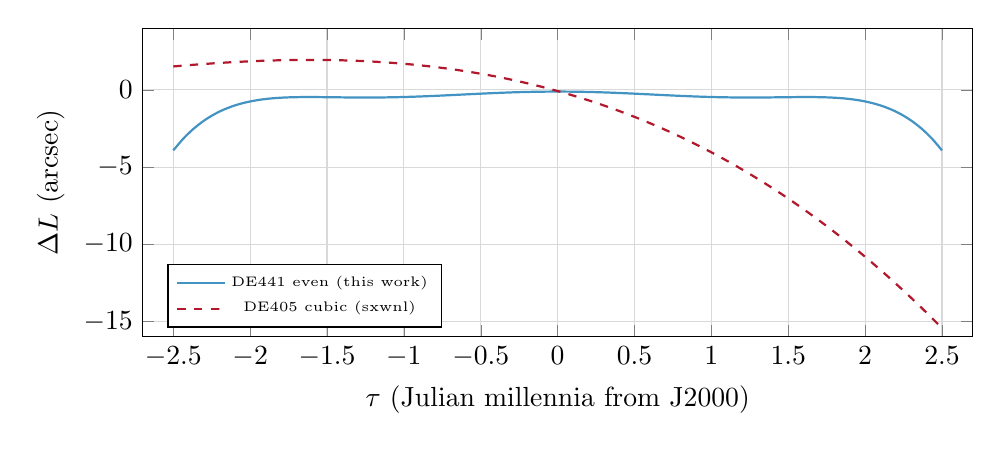
\begin{tikzpicture}
\begin{axis}[
    width=\columnwidth,
    height=5.5cm,
    xlabel={$\tau$ (Julian millennia from J2000)},
    ylabel={$\Delta L$ (arcsec)},
    xmin=-2.7, xmax=2.7,
    ymin=-16, ymax=4,
    grid=major,
    grid style={gray!30},
    legend pos=south west,
    legend style={font=\tiny},
]
\addplot[de441blue, thick, smooth, domain=-2.5:2.5, samples=80]
    {-0.1067 - 0.6166*x^2 + 0.3154*x^4 - 0.0503*x^6};
\addlegendentry{DE441 even (this work)}
\addplot[de405red, thick, dashed, smooth, domain=-2.5:2.5, samples=80]
    {-0.0728 - 2.7702*x - 1.1019*x^2 - 0.0996*x^3};
\addlegendentry{DE405 cubic (sxwnl)}
\end{axis}
\end{tikzpicture}
\caption{Correction polynomial comparison. The DE441 even sextic (solid) is
symmetric by construction; the DE405 cubic (dashed) diverges to $-15''$ for
future dates.}
\label{fig:correction}
\end{figure}

\subsection{Error~5: Historical $\Delta T$ Uncertainty}

\textbf{Magnitude: minutes to hours for ancient dates.}

\begin{table}[H]
\centering
\caption{$\Delta T$ uncertainty by epoch}
\label{tab:deltaT}
\footnotesize
\begin{tabular}{lrrl}
\toprule
\textbf{Epoch} & $\Delta T$ & \textbf{Unc.} & \textbf{Impact} \\
\midrule
1900 CE & $-2.7$~s & $<1$~s & Negl. \\
1600 CE & $+120$~s & $\sim 25$~s & $\sim 30$~s \\
1000 CE & $+1570$~s & $\sim 80$~s & $\sim 1.3$~min \\
500 CE & $+5710$~s & $\sim 200$~s & $\sim 3.3$~min \\
\bottomrule
\end{tabular}
\end{table}

This is \emph{irreducible}: no ephemeris improvement can compensate for
unknown historical Earth rotation \cite{stephenson2016}.


% =============================================================================
\section{The Reference Longitude Problem: A Cross-Civilizational Perspective}
\label{sec:meridians}

The question of \emph{which longitude to use as reference} for time-dependent
calculations is not unique to Chinese metaphysics. Every major astronomical
tradition confronted the same problem, and every civilization resolved it by
declaring its own center of the world. Understanding this pattern illuminates
why the \zh{洛陽} reference longitude debate (Section~\ref{subsubsec:luoyang})
is structurally inevitable rather than a mere historical curiosity.

\subsection{Axis Mundi: The Universal Claim to Centrality}
\label{subsec:axismundi}

The comparative religionist Mircea Eliade identified a near-universal pattern
he termed the \textit{axis mundi}: the belief that one's own location stands
at the center of the world, the point where heaven connects with
earth~\cite{eliade1958}. This impulse manifests in both sacred geography
and practical astronomy.

\begin{table}[H]
\centering
\caption{Sacred and astronomical centers across civilizations}
\label{tab:centers}
\footnotesize
\adjustbox{max width=\columnwidth}{%
\begin{tabular}{@{}llll@{}}
\toprule
\textbf{Civ.} & \textbf{Sacred Center} & \textbf{Astron.\ Ref.} & \textbf{Long.} \\
\midrule
Chinese    & \zh{洛陽} (\zh{天下之中})  & Dengfeng gnomon    & $113.07\degree$E \\
Indian     & Mt.~Meru (cosmic)         & Ujjain             & $75.77\degree$E \\
Greek      & Delphi (omphalos)         & Fortunate Isl.     & ${\sim}18\degree$W \\
Babylonian & Babylon (ziggurat)        & Babylon            & $44.42\degree$E \\
Islamic    & Mecca (Ka'aba)            & Baghdad / Ujjain   & $44.37\degree$E \\
Egyptian   & Heliopolis                & Alexandria         & $29.92\degree$E \\
\bottomrule
\end{tabular}}
\end{table}

A critical distinction separates two functions that are often conflated:

\begin{enumerate}[nosep]
  \item \textbf{Sacred center} (\textit{omphalos}): a mythological or
    religious claim about cosmic significance, requiring no instrumental
    verification.
  \item \textbf{Astronomical reference}: a practical origin point for
    coordinate-dependent calculations, requiring consistency but not
    uniqueness.
\end{enumerate}

\noindent
The Chinese \zh{天下之中} is unusual in that these two functions were
\emph{fused}: the same gnomon measurement that established Yangcheng (Dengfeng)
as the astronomical reference also served as the proof of its sacred centrality.
The criterion---an 8-\zh{尺} gnomon casting a 1.5-\zh{尺} shadow at noon on
the summer solstice---is simultaneously an empirical observation and a
cosmological claim~\cite{needham1959}.

\subsection{The Chinese Astronomical Meridian}
\label{subsec:chinese_meridian}

\subsubsection{The Duke of Zhou's Gnomon (\zh{周公測景台})}

The oldest layer of the Chinese reference meridian tradition dates to the
founding of the Zhou dynasty (c.~1046~BCE). The \textit{Zhou Li} records that
the Duke of Zhou (\zh{周公}) erected a gnomon at Yangcheng (\zh{陽城},
modern Gaocheng, Dengfeng, Henan; $34\degree 27' 31.5''$N,
$113\degree 04' 03.8''$E) to determine the ``center of heaven and earth.''
The original earthen gnomon (\zh{土圭}) was rebuilt in stone in 723~CE
(Tang dynasty, 11th year of Kaiyuan) by court astronomer Nangong Yue
(\zh{南宮說}), producing the surviving \zh{八尺表} (Eight-Chi Gnomon),
with gnomon and base each 1.98~m---exactly 8~\zh{尺} in Tang
metrology~\cite{needham1959}.

The stone gnomon was oriented so that on the summer solstice, it cast
\emph{no shadow beyond its base}, earning it the name \zh{無影台}
(``Shadowless Platform''). This zero-shadow condition was taken as
empirical proof of centrality.

\subsubsection{Yi Xing's Meridian Network (724~CE)}

The Tang dynasty astronomer Yi Xing (\zh{一行}, 683--727) constructed
20~standardized gnomons across China, with 10~aligned along the meridian
$114\degree$E from Central Asia to Vietnam---following a proposition by Liu
Zhuo (\zh{劉焯}) from 604~CE. This was an explicit attempt to measure
the Earth's circumference and to quantify how shadow lengths varied with
latitude~\cite{cullen1996}. The observations underpinned the Da Yan calendar
(\zh{大衍曆}). Yi~Xing's network represents one of the earliest systematic
geodetic surveys in any civilization.

\subsubsection{Guo Shoujing's Dengfeng Observatory (\zh{登封觀星台}, 1276)}

The culmination of the Chinese gnomon tradition came under the Yuan dynasty,
when Guo Shoujing (\zh{郭守敬}, 1231--1316) constructed a monumental
observatory at Gaocheng. Its 40-\zh{尺} ($\sim$12~m) gnomon was five times
the height of the traditional instrument, paired with a 31.9~m stone
measurement path (\zh{石圭}) comprising 36~stones with parallel waterways
for leveling. Guo established 27~observatories across the empire, from
the Yenisei River in Siberia to the South China Sea.

The resulting Shoushi calendar (\zh{授時曆}, 1281) determined the tropical
year as $365.2425$~days---identical to the value later adopted by the
Gregorian calendar (1582), but achieved three centuries
earlier~\cite{sivin2009}. Johann Adam Schall von Bell, encountering Guo's
instruments four centuries later, called him ``the Tycho Brahe of China.''

\subsubsection{The Shift to Beijing}

When the Ming dynasty (1368--1644) moved the capital to Beijing, the
practical astronomical reference shifted northeastward. Before 1913,
the official time standard for all of China was the \emph{apparent solar
time of Beijing}. The 1645 Shixian calendar reform (\zh{時憲曆}),
executed by the Jesuit Johann Adam Schall von Bell under Qing patronage,
further cemented Beijing as the computational center while introducing
Western trigonometric methods for ephemeris calculation. Matteo Ricci
(1552--1610) had already introduced the Western coordinate system and
fixed Beijing's latitude at $40\degree$N in his 1602 world map
(\zh{坤輿萬國全圖})~\cite{udias1994}.

\subsubsection{Modern China: UTC+8 and the $120\degree$E Standard}

In 1918, the Republic of China proposed five time zones spanning
UTC+5:30 to UTC+8:30~\cite{china_timezones_1918}. After 1949, Mao Zedong
abolished these in favor of a single UTC+8 standard (``Beijing
Time''), centered on the $120\degree$E meridian. China spans $73\degree$E to $135\degree$E---62~degrees of
longitude---meaning that solar noon in Kashgar ($76\degree$E) occurs at
approximately 15:10 clock time, a $176$-minute deviation from the standard
meridian (cf.~Error~4, Section~\ref{subsec:error4}).

The archaeological center (\zh{洛陽}/Dengfeng, ${\sim}113\degree$E), the
political center (Beijing, ${\sim}116.4\degree$E), and the time-zone center
($120\degree$E) are three distinct longitudes, separated by up to $7.55\degree$
($\approx 30$~min). For time-sensitive metaphysical calculations, the choice
among them is consequential.

\subsection{The Indian Astronomical Meridian: Ujjain}
\label{subsec:ujjain}

Indian Siddhantic astronomy provides the closest structural parallel to
the Chinese system. The \textit{Surya Siddhanta} (composed 4th--8th century
CE, encoding methods described as already ancient) defines a prime meridian
(\textit{rekha}, ``line'') running from Mount Meru (the North Pole) through
Ujjain (\zh{烏闍衍那}; $75.77\degree$E) to Lanka---not modern Sri Lanka,
but a theoretical point on the equator at zero latitude and zero
longitude~\cite{burgess1860}.

The \textit{Surya Siddhanta} (I.62) specifies that the following places
lie on this meridian: Rohitaka (Rohtak), Avanti (Ujjain), and Kurukshetra.
Three major astronomers anchored their work to this reference:

\begin{itemize}[nosep]
  \item \textbf{Aryabhata} (476--550~CE): defined the \textit{audayaka}
    system (day begins at sunrise at Lanka) and the \textit{ardha-ratrika}
    system (day begins at midnight at Lanka)~\cite{shukla1976}.
  \item \textbf{Brahmagupta} (c.~598--668~CE): composed the
    \textit{Brahmasphutasiddhanta} (628~CE) and eventually settled in
    Ujjain~\cite{plofker2009}.
  \item \textbf{Bhaskaracharya} (1114--1185~CE): refined Ujjain-based
    computations in the \textit{Siddhanta Shiromani}.
\end{itemize}

The operational mechanism for longitude correction was called
\textit{deshantara} (``difference of place''): once planetary positions were
computed for the Ujjain meridian, local almanacs (\textit{panchanga}) could be
derived by applying a correction proportional to the observer's longitude
offset from Ujjain. This is structurally identical to the modern formula
in Eq.~\eqref{eq:tst}, with Ujjain replacing $\phi_0 = 120\degree$E.

The \textit{Surya Siddhanta} also calculated Earth's diameter as 8,000~miles
(modern value: 7,928~miles) and positioned Ujjain at the intersection of
its prime meridian with the Tropic of Cancer~\cite{burgess1860}. Maharaja
Jai Singh~II built one of his five Jantar Mantar observatories at Ujjain
in 1725, explicitly because of the meridian's enduring significance.

\subsection{Ptolemy and the Fortunate Islands}
\label{subsec:ptolemy}

The Western astronomical tradition begins with Eratosthenes (c.~276--195~BCE),
who calculated the Earth's circumference at Alexandria, and Hipparchus
(c.~190--120~BCE), who developed the first geographic coordinate system at
Rhodes. Claudius Ptolemy (c.~90--168~CE) systematized their work in his
\textit{Geographia} (c.~150~CE), setting $0\degree$ longitude at the
``Fortunate Islands'' (\textit{Insulae Fortunatae})---identified with the
Canary Islands ($13\degree$--$18\degree$W)---to ensure all known lands had
positive longitudes, since negative numbers were not yet in
use~\cite{berggren2000}.

Ptolemy located Alexandria at $60\degree 30'$E from this meridian and
estimated the Earth's circumference at 180,000~stadia (${\sim}33{,}300$~km),
about 17\% less than the true value of 40,075~km. His maps spanned
$180\degree$ of longitude from the Canaries to China. Notably, Ptolemy
acknowledged the Indian astronomical center, recording ``Ozine'' (Ujjain) in
his gazetteer~\cite{berggren2000}.

The Fortunate Islands system persisted for over 1,500~years. In 1541,
Mercator drew his prime meridian through Fuerteventura ($14\degree 01'$W);
in 1634, Cardinal Richelieu fixed France's reference at El~Hierro, the
westernmost Canary island. The Ferro meridian remained in official Austrian
and German cartographic use well into the 20th~century.

\subsection{Islamic Astronomical Meridians}
\label{subsec:islamic}

Islamic astronomy inherited both the Ptolemaic and Indian traditions and
adapted them to new reference points. Al-Khwarizmi (c.~780--850~CE),
working at the Bayt al-Hikma (House of Wisdom) in Baghdad under Caliph
al-Ma'mun (r.~813--833), set his prime meridian at the eastern shore of
the Mediterranean---approximately $10\degree$--$13\degree$ east of
Ptolemy's Alexandria reference and $70\degree$ west of
Baghdad~\cite{kennedy1956}. He corrected Ptolemy's overestimate of the
Mediterranean from $63\degree$ to approximately $50\degree$ of longitude,
much closer to the true value.

Some Islamic astronomers, including al-Hamdani and Habash al-Hasib
al-Marwazi, adopted the Indian Ujjain meridian---evidence of direct
transmission of Indian astronomical methods through the Silk
Road~\cite{pingree1970}. The transmission went both ways: the Sanskrit
trigonometric term \textit{jya} (sine), the zero, the decimal place-value
system, and the astronomical works of Aryabhata and Brahmagupta all traveled
from India to Baghdad during al-Ma'mun's reign.

The Islamic tradition reached its observational pinnacle at Samarkand, where
Ulugh Beg (1394--1449) built an observatory with a 40-meter radius sextant
embedded in a meridian trench. Its graduation was so fine that
$1\degree = 70.2$~cm, $1' = 11.7$~mm, and $5'' = 1$~mm. The resulting
\textit{Sultani Zij} (1438--39) measured the tropical year to within
25~seconds of the true value---the most accurate determination before
Tycho Brahe~\cite{sayili1960}.

\subsection{The Greenwich Standardization}
\label{subsec:greenwich}

\subsubsection{The Longitude Problem and the Royal Observatory}

The Royal Observatory at Greenwich was founded on 22~June~1675 by King
Charles~II, with the explicit mandate of ``finding out the so much desired
Longitude of Places for perfecting the art of Navigation.'' The catalyst
was an embarrassing episode: a French astronomer, Sieur de St.~Pierre,
claimed to have solved the longitude problem using lunar distances. His
method was rejected, but the incident---facilitated by Charles's French
mistress Louise de K\'{e}roualle---highlighted England's lack of a national
observatory~\cite{sobel1995}.

John Flamsteed, appointed as the first Astronomer Royal on 4~March~1675,
made over 50,000~observations in 40~years, producing the
\textit{Historia Coelestis Britannica} (3,000~stars). The longitude
problem itself was not solved astronomically but mechanically, by John
Harrison's marine chronometer H4 (1760s), after Parliament offered a
\pounds 20,000 prize in 1714~\cite{sobel1995}.

\subsubsection{The 1884 International Meridian Conference}

Before 1884, over 25~prime meridians were in simultaneous use across
national observatories and cartographic traditions (Table~\ref{tab:meridians}).

\begin{table}[H]
\centering
\caption{Selected prime meridians in use before 1884}
\label{tab:meridians}
\small
\begin{tabular}{@{}llr@{}}
\toprule
\textbf{Meridian} & \textbf{Used by} & \textbf{$\Delta$ from Greenwich} \\
\midrule
Ferro (El Hierro)  & Austria, Germany       & $-17\degree 40'$ \\
Paris              & France                 & $+2\degree 20'$ \\
Pulkovo            & Russia                 & $+30\degree 20'$ \\
Cadiz              & Spain                  & $-6\degree 17'$ \\
Rome               & Italy                  & $+12\degree 27'$ \\
Copenhagen         & Denmark                & $+12\degree 34'$ \\
Stockholm          & Sweden                 & $+18\degree 03'$ \\
Washington         & United States          & $-77\degree 03'$ \\
Beijing            & China                  & $+116\degree 23'$ \\
\bottomrule
\end{tabular}
\end{table}

The International Meridian Conference convened in Washington, D.C., in October
1884, with 41~delegates from 25~nations. The key votes:

\begin{itemize}[nosep]
  \item \textbf{Resolution~1} (adopt a single meridian): \emph{unanimous}.
  \item \textbf{Resolution~2} (fix it at Greenwich): 22~ayes, 1~nay
    (San Domingo), 2~abstentions (\textbf{France} and Brazil).
  \item \textbf{Counter-proposal} (``neutral'' meridian cutting no great
    continent): 3~ayes, 21~nays.
\end{itemize}

\noindent
Greenwich prevailed because 72\% of global shipping tonnage already used it
as zero longitude~\cite{howse1997}. France abstained on principle, arguing that a prime
meridian should have ``a character of absolute neutrality''---a position
undermined by France's simultaneous insistence on the metric system, which
was itself a French creation.

France did not adopt Greenwich on its maps until 1911, and even then the
enabling legislation referred to the new standard as ``\textit{l'heure de
temps moyen de Paris, retard\'{e}e de 9~minutes 21~secondes}'' (``the mean
time of Paris, retarded by 9~minutes 21~seconds''), carefully avoiding any
mention of Greenwich or England~\cite{howse1997}. The confusion of competing
meridians had real consequences: when the \textit{Titanic} sank in April~1912,
the inquiry revealed that the French vessel \textit{La Touraine} had sent an
ice warning with times on the Greenwich meridian but longitudes on the Paris
meridian.

\subsection{Megalithic and Mesoamerican Traditions}
\label{subsec:megalithic}

Not all astronomical traditions developed longitude-based reference systems.
The megalithic builders of northwestern Europe (Stonehenge, c.~3000--2000~BCE;
Newgrange, c.~3200~BCE) and the Maya astronomers of Mesoamerica (El~Caracol
at Chich\'{e}n Itz\'{a}, c.~AD~906) employed \emph{horizon-based} reference
systems---alignments to specific azimuths of solstice sunrise, equinox sunset,
or Venus elongations---rather than coordinate grids.

Newgrange's roof box, which admits sunlight to the inner chamber for exactly
17~minutes on the winter solstice, demonstrates precision comparable to
gnomon-based systems but encodes information architecturally rather than
numerically~\cite{patrick1974}. The Maya at El~Caracol tracked Venus's
synodic cycle with sufficient accuracy to predict its extreme elongations;
their calculation of the synodic month exceeded Ptolemy's in
precision~\cite{aveni2001}. However, the absence of a coordinate-grid
framework means these traditions did not generate the ``which meridian?''
problem inherent in coordinate-dependent systems like \zh{紫微斗數}.

\subsection{The Anthropological Pattern}
\label{subsec:pattern}

The cross-civilizational evidence reveals a consistent three-stage pattern:

\begin{enumerate}
  \item \textbf{Sacred center}: A location is declared the cosmic
    center---\zh{天下之中}, Delphi's omphalos, Babylon's ziggurat,
    Mecca's Ka'aba---on mythological or theological grounds.
  \item \textbf{Astronomical reference}: The sacred center acquires
    practical function as the zero point for coordinate-dependent
    calculations (Ujjain's \textit{deshantara}, Dengfeng's gnomon,
    Ptolemy's Fortunate Islands).
  \item \textbf{Political standardization}: Competing references are
    resolved by political consensus rather than scientific argument
    (1884 Conference, 1949 Beijing Time decree).
\end{enumerate}

\noindent
The choice of reference meridian is therefore \emph{always} a political
act, regardless of its scientific packaging. China's name for
itself---\zh{中國}, ``Middle Kingdom''---encodes the same ethnocentric
cartographic impulse that led every other civilization to place itself
at the center of its maps~\cite{harley1987}.

For Chinese metaphysical computation, this analysis yields a concrete
conclusion: there is no ``correct'' reference longitude, only
\emph{historically appropriate} ones. Software computing a chart for
a Tang-dynasty birth should arguably use the Dengfeng meridian
($113.07\degree$E); for the Ming and Qing, Beijing ($116.4\degree$E);
for modern births, the UTC+8 standard ($120\degree$E). The $\sim 30$-minute
maximum difference between these references
($(120 - 113.07) \times 4 \approx 28$~min) is large enough to shift
the \zh{時辰} boundary for approximately 4.2\% of births
(those within 28~minutes of a double-hour boundary).

\subsection{The Celestial Reference Frame: Tropical vs.\ Sidereal}
\label{subsec:tropical_sidereal}

The preceding sections examined reference-frame problems in spatial
coordinates (which meridian?) and temporal coordinates (apparent vs.\
mean vs.\ zone time).  A third reference-frame problem, equally
consequential for Chinese metaphysics, operates in celestial
coordinates: the choice between a \emph{tropical} zodiac (anchored to
the vernal equinox) and a \emph{sidereal} zodiac (anchored to fixed
stars).

The two frames coincided approximately in the early centuries~CE.
Because Earth's rotational axis precesses with a period of
$\sim$25,772~years, the vernal equinox drifts westward along the
ecliptic at $\sim 50.3''$/year ($\approx 1.4\degree$/century) relative
to the fixed stars~\cite{needham1959}.  By 2026, the cumulative offset
(the \emph{ayanamsa}) is $\approx 24\degree\,10'$ in the standard
Lahiri system---nearly one full zodiacal division of
$30\degree$~\cite{chandra_hari_1998}.

\textbf{Chinese independent discovery of precession.}
The Chinese discovery of precession was independent of Hipparchus
(c.~190--120~BCE).  Yu~Xi (\zh{虞喜}, c.~281--356~CE, Eastern Jin
dynasty) observed in his \zh{安天論} (\textit{An Tian Lun},
``Disquisition on the Conformation of the Heavens,'' 336~CE) that the
winter solstice position had drifted $\sim 1\degree$ per 50~years
relative to the stars---overestimating the true rate
($1\degree/71.6$~yr) by $\sim$44\%, but correctly identifying the
phenomenon~\cite{needham1959, hockey_bea_2014}.  Zu~Chongzhi
(\zh{祖沖之}, 429--501~CE) was the first to incorporate precession into
calendar calculations in his \zh{大明曆} (Daming Calendar).

\textbf{Which systems use which frame?}
The five systems discussed in this paper split across both frames:
\begin{itemize}[nosep]
  \item \textbf{Tropical}: \zh{八字} and \zh{奇門遁甲} (via solar
    terms, defined by the Sun's tropical longitude); \zh{大六壬}'s
    modern \zh{中氣換將法} method.
  \item \textbf{Sidereal}: \zh{七政四餘} (28~\zh{宿} tied to
    determinative stars~\cite{sun_kistemaker_1997}); \zh{大六壬}'s
    historical \zh{日躔法} (Sun's position in 12 sidereal
    \zh{星次}).
  \item \textbf{Hybrid}: \zh{紫微斗數} avoids the question entirely
    by using the lunar calendar date---a discrete quantity that
    inherits its tropical dependence from the intercalation
    algorithm without ever querying a zodiacal position.
\end{itemize}

\textbf{The ayanamsa controversy.}
For sidereal systems, the choice of zero point is not
physically determined.  Different traditions anchor the sidereal
zodiac to different reference stars, yielding different ayanamsas:
\begin{center}
\footnotesize
\begin{tabular}{lll}
\toprule
\textbf{System} & \textbf{Zero epoch} & \textbf{Notes} \\
\midrule
Lahiri (Citrapaksha) & 285~CE & Official Indian standard since 1955 \\
Fagan-Bradley & 221~CE & Western siderealist school \\
Raman & varies & $\sim 2\degree$ from Lahiri \\
Chinese 28~\zh{宿} & varies & Unequal widths, multiple epochs \\
\bottomrule
\end{tabular}
\end{center}
\noindent
The controversy is fundamentally irresolvable: no physically privileged
zero point exists for the sidereal
zodiac~\cite{chandra_hari_1998}.  The practical consequence is that
two software implementations using the same birth data, the same
ephemeris, and the same sidereal framework can still disagree on
mansion placements if they adopt different ayanamsas.

\textbf{The parallel with Indian Jyotish.}
The structural parallel between Chinese \zh{七政四餘} and Indian
Jyotish (\textit{Jyoti\d{h}\'{s}\={a}stra}) is instructive: both are
sidereal systems that require real planetary positions, both face the
ayanamsa problem, and both have adopted the Swiss Ephemeris for modern
computation~\cite{pingree_jyotihsastra}.  The key difference is that
Jyotish has a single dominant ayanamsa (Lahiri, mandated by the Indian
government since 1955), while the Chinese 28~\zh{宿} system never
achieved similar standardization---each historical star catalogue
(Shi~Shen \zh{石申}, Gan~De \zh{甘德}, Wu~Xian \zh{巫咸}) defines
slightly different mansion boundaries~\cite{sun_kistemaker_1997}.

\textbf{Ptolemy and the Western tropical choice.}
Western astrology adopted the tropical zodiac following Ptolemy's
\textit{Tetrabiblos} (c.~150~CE), which explicitly anchored the zodiac
to the vernal equinox: ``they assume that the sign which begins with
the vernal equinox, that of Aries, is the starting-point of them
all''~\cite{ptolemy_tetrabiblos}.  This was a deliberate choice---Ptolemy
was fully aware of precession from Hipparchus's work, discussed in his
\textit{Almagest}~\cite{toomer_almagest}.  The tropical choice made
Western astrology immune to precession drift but severed it from the
stellar constellations whose names it retained.  By 2026, the Sun
enters the tropical sign of Aries at the vernal equinox while
physically located in the constellation
Pisces---a $\sim 24\degree$ discrepancy that the sidereal tradition
considers a fundamental error and the tropical tradition considers
irrelevant.

\textbf{Computational implications.}
For Chinese metaphysical software, the tropical-sidereal distinction
creates the same category of error as the meridian problem: a
systematic offset that grows linearly with time.  The spatial
reference-frame error (meridian choice) is bounded at
$\sim$30~minutes of time ($7\degree$ longitude within China); the
celestial reference-frame error (ayanamsa) is bounded only by the
epoch range under consideration, reaching $\sim 28\degree$ over two
millennia.  For \zh{七政四餘} mansion placements, where mansion widths
range from $<1\degree$ to $\sim 33\degree$, an uncorrected
$24\degree$~ayanamsa can shift a planet across multiple mansion
boundaries---an error far larger than any ephemeris imprecision.

\subsection{Computational Implications: Three Time Regimes}
\label{subsec:timeregimes}

The historical transition from local apparent solar time to standardized
zone time introduced three distinct regimes, each with different error
characteristics for Chinese calendrical computation:

\begin{enumerate}
  \item \textbf{Local Apparent Solar Time} (pre-17th century):
    Historical users relied on sundials, so their ``time'' was
    automatically local and apparent. No longitude correction was
    needed, but the Equation of Time ($\pm 16$~min) was implicitly
    absorbed. Reconstructing such charts requires computing true local
    solar time for the birth location.

  \item \textbf{Local Mean Solar Time} (17th--19th century):
    With the adoption of mechanical clocks, mean solar time replaced
    apparent solar time. The Equation of Time became an explicit
    correction. Ptolemy had already tabulated it in the 2nd century CE
    (\textit{Almagest} Book~III and \textit{Handy Tables}), but it only
    became practically relevant when clocks, rather than sundials,
    became the primary timekeeping instruments.

  \item \textbf{Standard Zone Time} (post-1884, post-1949 in China):
    The adoption of UTC+8 across all of China introduced a longitude
    correction of up to $4 \times (120 - \phi)$~minutes, where $\phi$
    is the local longitude. Combined with the Equation of Time, the
    total correction from clock time to true local solar time can reach:
    \[
      |\Delta t_{\max}| = |(\phi - 120) \times 4| + 16 \approx 192~\text{min}
    \]
    for Kashgar ($\phi = 76\degree$E), placing a midnight birth nearly
    3.2~hours earlier in true solar time.
\end{enumerate}

\noindent
The Shanghai--Chengdu comparison illustrates the practical impact.
Both cities use UTC+8, but Shanghai ($121.47\degree$E) sits near the
zone center while Chengdu ($104.07\degree$E) is $15.93\degree$ west:

\begin{align}
  \Delta t_{\text{Shanghai}} &= (121.47 - 120) \times 4 = +5.9~\text{min} \\
  \Delta t_{\text{Chengdu}}  &= (104.07 - 120) \times 4 = -63.7~\text{min}
\end{align}

\noindent
A birth recorded as 23:15 clock time yields:
\begin{itemize}[nosep]
  \item Shanghai: ${\sim}23{:}21$ local solar time $\to$ \zh{子時}
    (Zi hour, 23:00--01:00)
  \item Chengdu: ${\sim}22{:}11$ local solar time $\to$ \zh{亥時}
    (Hai hour, 21:00--23:00)
\end{itemize}

\noindent
The same clock time produces \emph{different hour pillars}---and potentially
different day pillars if the Zi hour boundary is crossed---despite
identical civil timestamps. Adding the Equation of Time ($\pm 16$~min
depending on date of birth) can push borderline cases across yet another
boundary.


% =============================================================================
\section{Historical Uncertainty}
\label{sec:uncertainty}

\subsection{$\Delta T$ and Earth Rotation}
\label{subsec:deltaT}

The long-term $\Delta T$ trend is driven by tidal friction (LOD increase
$+2.3$~ms/century), partially offset by post-glacial rebound
($-0.6$~ms/century), yielding an observed $+1.8$~ms/century
\cite{stephenson2016}; earlier eclipse-based constraints appear in
\cite{stephenson1986}. Before $\sim$1600~CE, $\Delta T$ uncertainty
dominates all other error sources by 1--2 orders of magnitude.

\subsection{The Little Ice Age and Maunder Minimum}

The Little Ice Age ($\sim$1300--1850~CE)---documented in
\zh{竺可楨}'s landmark study of Chinese climate over five
millennia~\cite{zhukz1973}---was contemporaneous with the Sp\"{o}rer
(1450--1550) and Maunder (1645--1715) Minima of solar activity
\cite{eddy1976}. While climate does not directly affect astronomical
computation, the Maunder Minimum disrupted European telescopic observations.
Chinese naked-eye sunspot records continued---23 independent observations in
1618 alone \cite{hayakawa2022}---providing the only pre-telescopic solar
activity constraints. Hayakawa et~al.\ have also catalogued 270 sunspot
and aurora candidates in Chinese official histories from the late Song
through Ming dynasties (1261--1644)~\cite{hayakawa2017}.

\subsection{Eclipse Records}

Chinese eclipse records serve dual purposes: constraining $\Delta T$ before
the telescopic era \cite{stephenson2018}, and validating the entire
computational pipeline. A 2025 re-analysis of the 709~BCE eclipse---humanity's
earliest datable total solar eclipse recorded in Chinese annals---refined
measurements of 8th-century~BCE rotational deceleration
\cite{eclipse709bce_2025}.

\subsection{Error Budget by Epoch}

\begin{figure}[H]
\centering
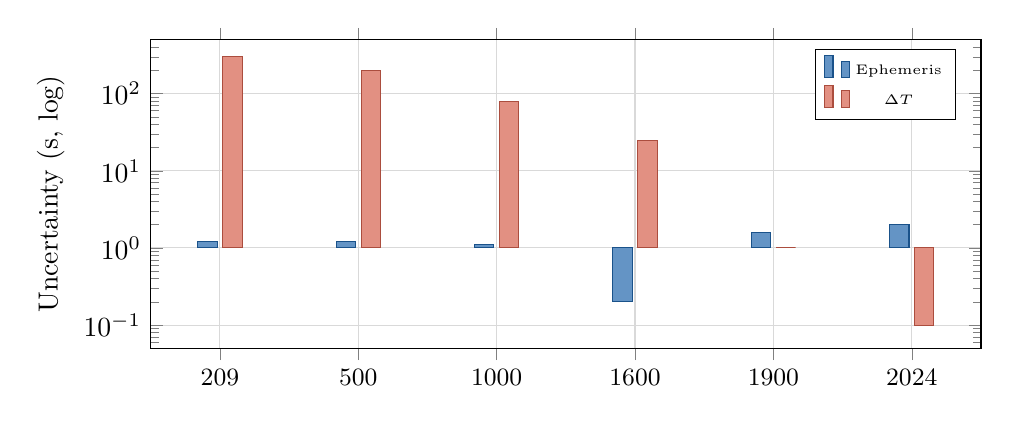
\begin{tikzpicture}
\begin{axis}[
    width=\columnwidth,
    height=5.5cm,
    ybar,
    bar width=7pt,
    ylabel={Uncertainty (s, log)},
    ymode=log,
    log basis y=10,
    ymin=0.05, ymax=500,
    symbolic x coords={209,500,1000,1600,1900,2024},
    xtick=data,
    xticklabel style={font=\small},
    grid=major,
    grid style={gray!30},
    legend pos=north east,
    legend style={font=\tiny},
]
\addplot[fill=sbblue!70, draw=sbblue!80!black] coordinates {
    (209,1.2) (500,1.2) (1000,1.1) (1600,0.2) (1900,1.6) (2024,2.0)
};
\addlegendentry{Ephemeris}
\addplot[fill=sxorange!70, draw=sxorange!80!black] coordinates {
    (209,300) (500,200) (1000,80) (1600,25) (1900,1) (2024,0.1)
};
\addlegendentry{$\Delta T$}
\end{axis}
\end{tikzpicture}
\caption{Error budget decomposition (log scale). $\Delta T$ exceeds ephemeris
error by 1--2 orders of magnitude before $\sim$1600~CE.}
\label{fig:error_budget}
\end{figure}

\textbf{Implication}: For a historical figure born in 500~CE, $\Delta T$
uncertainty ($\sim 200$~s $\approx 3.3$~min) is $\sim 200\times$ larger than
ephemeris error ($\sim 1$~s). Sub-minute precision claims for ancient charts
are physically meaningless.

% =============================================================================

% =============================================================================
\section{Competing Calendar Authorities}
\label{sec:authorities}

The errors catalogued above---ephemeris precision, true solar time, DST---are
\emph{technical} problems with deterministic solutions.  A qualitatively
different class of error arises from the fact that there is no single,
universally accepted authority for the Chinese calendar and its derived
metaphysical computations.  Multiple institutions and lineages publish
calendars that disagree on specific dates, and users downstream
inherit whichever source their software or almanac chose.

\subsection{The Official Authority: \zh{紫金山天文台}}
\label{subsec:pmo}

Purple Mountain Observatory (PMO, \zh{紫金山天文台}) in Nanjing has served
as the sole official calendar authority for the People's Republic of China
since 1949, inheriting a mandate that traces to the Academia Sinica's
adoption of the site in 1929~\cite{hko_calendar_history}.  PMO computes solar terms using \zh{定氣}
(true ecliptic longitude) referenced to UTC$+$8 at $120\degree$E, with
ephemeris data drawn from JPL~DE441~\cite{jpl_de441}---though the
\textit{Chinese Astronomical Almanac} was still using DE421 as of 2025,
a difference negligible for recent centuries.

The national standard GB/T~33661-2017~\cite{gbstandard2017} codifies this
arrangement, mandating approximately one-second accuracy for solar term and
new moon calculations and designating PMO as the sole official publisher of
the \zh{農曆}.  Prior to 1984, PMO relied on Newcomb's Tables
(1895)~\cite{meeus1998}, introducing systematic solar term timing errors
of approximately 25~seconds relative to modern ephemerides.

A recent development is the LTE440 lunar timekeeping ephemeris published
in \textit{Astronomy \& Astrophysics} (2025)~\cite{pmo_lte440}, extending
PMO's computational infrastructure to high-precision lunar timescales.

\subsection{The Traditional Authority: \zh{蔡真步堂}}
\label{subsec:choibooks}

The \zh{蔡真步堂} (Choi Chan Po Tong) lineage represents the most
commercially significant traditional calendar authority in the Chinese
world, with over 70~million copies of its almanacs
sold~\cite{scmp_choi_obituary} through publishers \zh{永經堂} and
\zh{廣經堂}.  The lineage spans four generations
(Table~\ref{tab:choi_lineage}).

\begin{table}[H]
\centering
\caption{The \zh{蔡真步堂} lineage}
\label{tab:choi_lineage}
\small
\adjustbox{max width=\columnwidth}{%
\begin{tabular}{@{}llp{4cm}@{}}
\toprule
\textbf{Gen.} & \textbf{Name} & \textbf{Period / Notes} \\
\midrule
Founder    & \zh{蔡最白}  & Late Qing \zh{欽天監}; founded \zh{真步堂} 1891 \\
Second     & \zh{蔡廉仿}  & Republican era \\
Third      & \zh{蔡伯勵}  & 1922--2018; GBS (HKSAR) \\
Fourth     & \zh{蔡興華}  & Current; daughter of \zh{蔡伯勵} \\
\bottomrule
\end{tabular}}
\end{table}

\noindent
\zh{蔡興華}'s public statement---``We have no special techniques
\ldots\ the rules are basic compilation principles anyone can
self-study''~\cite{initium_choi_2019}---underscores that the expertise inherited from the
\zh{欽天監} is one of \emph{editorial judgment}, not secret algorithms.
Indeed, what was inherited from the \zh{欽天監} was itself already a
Jesuit--European hybrid.  The post-1645 Shixian (\zh{時憲曆}) reform
introduced Tychonic planetary models, Western trigonometry, and the
\zh{定氣法} (true-longitude solar terms) into the imperial astronomical
bureau~\cite{udias1994, sivin2009}.  The ``traditional Chinese computation''
transmitted through \zh{真步堂} was thus fundamentally Western astronomy in
Chinese computational dress.

The \zh{蔡真步堂} almanac architecture comprises four layers:
\begin{enumerate}[nosep]
  \item \textbf{Calendar backbone}: post-1978, aligned with PMO
    calculations for solar terms and new moons.
  \item \textbf{\zh{七政經緯}}: planetary positions mapped into the
    28~lunar mansions (\zh{二十八宿}); see
    Section~\ref{subsec:qzsy} for the \zh{七政四餘} system.
  \item \textbf{\zh{擇日} (date selection)}: rules drawn primarily from
    the \zh{協紀辨方書}~\cite{xieji_bianfang}.
  \item \textbf{Editorial judgment}: filtering contradictions between
    competing date-selection schools.
\end{enumerate}

\noindent
It bears emphasis that \zh{真步堂} is not itself a publisher---\zh{永經堂}
and \zh{廣經堂} are the publishing houses that distribute almanacs computed
using \zh{真步堂} calculations.  The tradition was recognized as Guangdong
provincial-level intangible cultural heritage in
2013~\cite{choi_intangible}.

\subsection{\zh{協紀辨方書}: The Imperial Standard}
\label{subsec:xieji}

The full title \zh{欽定協紀辨方書} (``Imperially Endorsed Treatise on
Harmonizing Times and Distinguishing Directions'') signals the work's
dual purpose: to systematize the contradictory date-selection traditions
that had proliferated across centuries, and to explicitly debunk baseless
superstitions that had accreted around them.

Commissioned by the Qianlong Emperor and compiled under the supervision
of Prince Yun Lu (\zh{允祿}), the treatise was completed in 1739 and
comprises 36~\zh{卷} organized into 11~parts~\cite{xieji_bianfang}.
It was included in the \zh{四庫全書} and remains the foundation of all
modern \zh{通勝} (almanac) traditions---though many modern
almanacs subsequently reintroduced the very superstitions that the
\zh{協紀辨方書} had systematically excised.

A partial English translation is available as Thomas~F. Aylward's
\textit{The Imperial Guide to Feng Shui and Chinese
Astrology}~\cite{aylward2007}.

\subsection{The Fragmentation Problem}
\label{subsec:fragmentation}

The absence of a single authority has produced substantial regional
divergence.  In Taiwan alone, approximately 90~competing \zh{通勝} are
published annually~\cite{huang_tungshu}, of which over two-thirds trace
their lineage to the \zh{繼成堂} of Quanzhou, founded by \zh{洪潮和}.
The post-Cultural-Revolution period saw the PRC ban \zh{通勝} printing
entirely; when the prohibition was relaxed, the parent tradition had
collapsed, spawning numerous ``lesser brands'' with varying computational
fidelity.

\begin{table}[H]
\centering
\caption{Regional calendar authorities}
\label{tab:authorities}
\small
\adjustbox{max width=\columnwidth}{%
\begin{tabular}{@{}lll@{}}
\toprule
\textbf{Region} & \textbf{Authority} & \textbf{Status} \\
\midrule
Mainland China & PMO & Official; GB/T~33661 \\
Hong Kong      & HKO + \zh{蔡真步堂} & Dual system \\
Taiwan         & CWA + ${\sim}90$ \zh{通勝} & Fragmented \\
Overseas       & Mixed sources & No standard \\
\bottomrule
\end{tabular}}
\end{table}

\noindent
Eight distinct sources of disagreement between these authorities can be
identified:

\begin{enumerate}[nosep]
  \item \textbf{Reference meridian}: pre-1929 Beijing
    ($116\degree 25'$E) vs.\ modern standard ($120\degree$E)---a
    ${\sim}14$~minute time difference.
  \item \textbf{Timezone}: UTC$+$8 vs.\ UTC$+$9 (Korea, Japan) can shift
    new moon dates across midnight.
  \item \textbf{Ephemeris accuracy}: Newcomb (1895) vs.\ JPL~DE441 introduces
    systematic offsets in solar term timing.
  \item \textbf{Midnight boundary cases}: near-midnight astronomical events
    combined with calculation precision differences yield different calendar
    dates.
  \item \textbf{\zh{平氣} vs.\ \zh{定氣}}: the pre-1645 equal-interval
    method vs.\ the post-1645 true-longitude method produces different solar
    term dates and creates ``fake leap months''~\cite{aslaksen_fake}.
  \item \textbf{\zh{閏月} assignment rules}: even within \zh{定氣},
    the intercalary month algorithm admits edge cases where different
    implementations disagree.
  \item \textbf{\zh{擇日} methodology}: competing date-selection schools
    (e.g., \zh{洪潮和} vs.\ \zh{蔡真步堂}) apply different subsets of
    the \zh{協紀辨方書} rules.
  \item \textbf{Zombie superstitions}: methods that the
    \zh{協紀辨方書} explicitly debunked but that publishers retained for
    commercial or traditional reasons.
\end{enumerate}

\subsection{The 1978 Unification and Its Limits}
\label{subsec:unification1978}

The pivotal event was the 1978 Mid-Autumn Festival discrepancy~\cite{ytliu_rules}.
The relevant new moon fell at 00:07 CST on 3~September~1978 when computed for
the modern standard meridian ($120\degree$E), but at 23:53 on
2~September~1978 when computed for the old Beijing meridian
($116\degree 25'$E).  The result: Hong Kong celebrated the Mid-Autumn
Festival on 16~September while the mainland observed it on 17~September---a
visible public embarrassment that forced alignment.  Hong Kong subsequently
adopted PMO calculations for its calendar backbone.

However, this unification extended only to the astronomical
layer---solar terms, new moons, and the derived calendar structure.  The
\zh{擇日} interpretation layer, which determines which days are auspicious
or inauspicious for specific activities, remains fragmented across competing
schools and lineages.

A more subtle problem is the 2033 intercalary month.  Until the early
1990s, \emph{all} published Chinese calendars worldwide placed the 2033
leap month after month~7 rather than after month~11---an error that
persisted for decades before being
corrected~\cite{aslaksen_fake, wikipedia_2033}.  The root cause traces to
the Jesuits' 1645 \zh{定氣} reform: the switch from equal-interval
(\zh{平氣}) to true-longitude (\zh{定氣}) solar terms introduced
``fake leap months'' (\zh{偽閏月}) that do not arise under the older
system.  This is historically ironic---the \zh{定氣} method was introduced
partly to demonstrate the superiority of European astronomy over Chinese
methods, yet it created anomalies so confusing that even the Jesuits
themselves were jailed during the Calendar Case (\zh{曆獄}, 1664--1669, during the Oboi regency;
reversed by the Kangxi Emperor upon assuming personal rule), in
part because of these discrepancies~\cite{sivin2009, udias1994}.

% =============================================================================

% =============================================================================
\section{The Computational Pipeline}
\label{sec:background}

\subsection{Solar Term Definition}

Under the \zh{定氣} (\textit{d\`{i}ng q\`{i}}) method, adopted by the
Shixian calendar (\zh{時憲曆}) in 1645, each solar term is the instant when
the Sun's \emph{apparent} geocentric ecliptic longitude reaches a specific
multiple of $15\degree$ \cite{aslaksen2010, ytliu_rules}. This replaced the
\zh{平氣} method, which divided the tropical year into 24 equal time
intervals \cite{ytliu_solarterms}.

Because Earth's orbit is elliptical ($e \approx 0.0167$), the Sun's ecliptic
longitude does not advance uniformly: $\sim 1.02\degree$/day near perihelion
vs.\ $\sim 0.95\degree$/day near aphelion~\cite{meeus1998}.

\subsection{Computational Pipeline}
\label{subsec:pipeline}

The Sun's apparent ecliptic longitude $\lambda_\odot$ is computed as:

\begin{equation}
  \lambda_\odot = \lambda_{\text{geo}} + \Delta\psi + \Delta\tau_{\text{ab}}
  \label{eq:apparent}
\end{equation}

\noindent where $\lambda_{\text{geo}} = L + 180\degree$ (geocentric from
heliocentric Earth longitude $L$ via VSOP87D \cite{bretagnon1988}),
$\Delta\psi$ is nutation in longitude (IAU2000B, 77 terms \cite{iau2000b}),
and $\Delta\tau_{\text{ab}} = -20.4898'' / R$ is aberration~\cite{ronvondrak1986}.

Three time scales are relevant: TT (Terrestrial Time, uniform), UT (Universal
Time, based on Earth rotation), and $\Delta T = \text{TT} - \text{UT}$
($\approx 69.1$~s for mid-2024)~\cite{nasa_deltaT_uncertainty, stephenson2016}.

% =============================================================================

% =============================================================================
\section{Statistical Validation}
\label{sec:validation}

\subsection{Methodology}

Three-way comparison between: (1)~\textbf{stem-branch} (VSOP87D + DE441
correction + IAU2000B), (2)~\textbf{sxwnl} (VSOP87D + DE405 cubic +
ELP/MPP02) \cite{sxwnl_github}, and (3)~\textbf{JPL Horizons} (DE441
numerical integration) \cite{jpl_horizons}. The computational methodology
for the Chinese calendar follows Liu~\cite{ytliu_computation}.

42~sample years span 209--2493~CE (1,008 total solar terms). 12 systematic
years at 20-year intervals (1900--2100); 30 pseudo-random years (seed=42)
from 200--2800~CE.

\subsection{Equation of Time}
\label{subsec:eot}

366 daily samples at 12:00~TT across 2024:

\begin{table}[H]
\centering
\caption{EoT residuals: stem-branch vs.\ JPL (2024)}
\label{tab:eot}
\footnotesize
\begin{tabular}{lr}
\toprule
\textbf{Statistic} & \textbf{Value} \\
\midrule
Mean bias & $+0.000$~min \\
Mean $|\text{res.}|$ & 0.01~s \\
Std.\ dev. & 0.02~s \\
Max $|\text{res.}|$ & 0.03~s \\
\bottomrule
\end{tabular}
\end{table}

The 0.03~s maximum is a $\sim$1,000$\times$ improvement over the Spencer
(1971) Fourier approximation \cite{spencer1971}.

\begin{figure}[H]
\centering
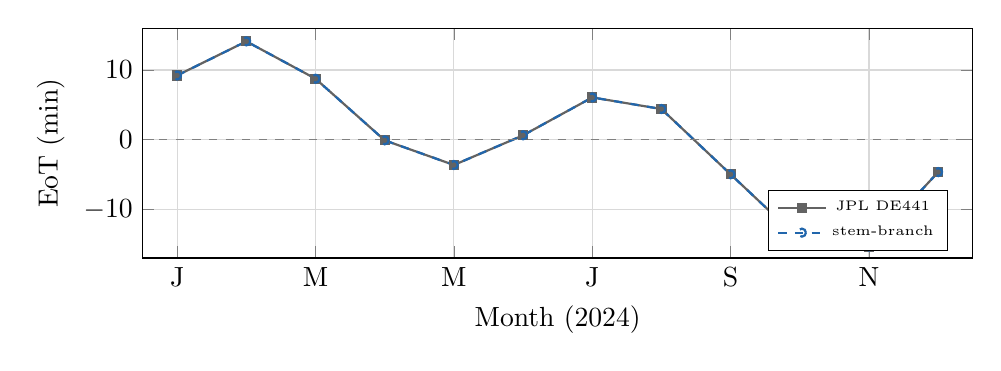
\begin{tikzpicture}
\begin{axis}[
    width=\columnwidth,
    height=4.5cm,
    xlabel={Month (2024)},
    ylabel={EoT (min)},
    xmin=0.5, xmax=12.5,
    ymin=-17, ymax=16,
    xtick={1,3,5,7,9,11},
    xticklabels={J,M,M,J,S,N},
    grid=major,
    grid style={gray!30},
    legend pos=south east,
    legend style={font=\tiny},
    mark size=1.8pt,
]
\addplot[jplgray, thick, mark=square*, mark options={fill=jplgray, scale=0.8}]
    coordinates {
        (1,9.22) (2,14.11) (3,8.75) (4,-0.10)
        (5,-3.64) (6,0.62) (7,6.06) (8,4.40)
        (9,-4.98) (10,-14.35) (11,-15.35) (12,-4.66)
    };
\addlegendentry{JPL DE441}
\addplot[sbblue, thick, dashed, mark=o, mark options={sbblue, scale=0.8}]
    coordinates {
        (1,9.22) (2,14.11) (3,8.75) (4,-0.10)
        (5,-3.64) (6,0.62) (7,6.06) (8,4.40)
        (9,-4.98) (10,-14.35) (11,-15.35) (12,-4.66)
    };
\addlegendentry{stem-branch}
\draw[gray, thin, dashed] (axis cs:0.5,0) -- (axis cs:12.5,0);
\end{axis}
\end{tikzpicture}
\caption{EoT annual profile (2024). The two sources are indistinguishable at
this resolution; maximum residual is 0.03\,s.}
\label{fig:eot}
\end{figure}

\subsection{Solar Term Timing}
\label{subsec:solarterms}

\begin{table}[H]
\centering
\caption{Solar term accuracy (seconds)}
\label{tab:accuracy}
\footnotesize
\begin{tabular}{lccccc}
\toprule
& $N$ & Mean & Max & P50 & P95 \\
\midrule
\multicolumn{6}{l}{\textit{Modern (1900--2100):}} \\
SB vs JPL & 336 & 1.56 & 2.79 & 1.68 & 2.29 \\
SX vs JPL & 335 & 2.38 & 7.18 & 1.85 & 5.71 \\
\midrule
\multicolumn{6}{l}{\textit{Full range (209--2493):}} \\
SB vs JPL & 1008 & 1.05 & 3.05 & 0.97 & 2.22 \\
\bottomrule
\end{tabular}
\end{table}

\begin{figure*}[t]
\centering
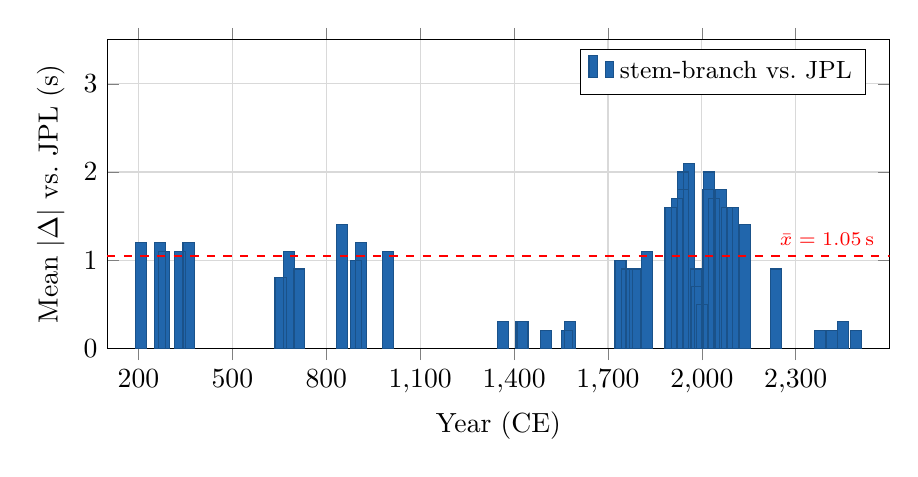
\begin{tikzpicture}
\begin{axis}[
    width=0.95\textwidth,
    height=5.5cm,
    ybar,
    bar width=4pt,
    xlabel={Year (CE)},
    ylabel={Mean $|\Delta|$ vs.\ JPL (s)},
    xmin=100, xmax=2600,
    ymin=0, ymax=3.5,
    grid=major,
    grid style={gray!30},
    xtick={200,500,800,1100,1400,1700,2000,2300},
    legend pos=north east,
    legend style={font=\small},
]
\addplot[fill=sbblue, draw=sbblue!80!black] coordinates {
    (209,1.2) (270,1.2) (281,1.1) (333,1.1) (360,1.2)
    (654,0.8) (682,1.1) (712,0.9) (849,1.4) (894,1.0)
    (910,1.2) (998,1.1)
    (1365,0.3) (1424,0.3) (1428,0.3) (1501,0.2) (1569,0.2) (1578,0.3)
    (1740,1.0) (1762,0.9) (1787,0.9) (1824,1.1)
    (1900,1.6) (1920,1.7) (1940,1.8) (1941,2.0) (1960,2.1)
    (1980,0.9) (1985,0.7) (2000,0.5) (2020,1.8) (2024,2.0)
    (2040,1.7) (2060,1.8) (2080,1.6) (2100,1.6)
    (2138,1.4) (2237,0.9) (2377,0.2) (2416,0.2) (2450,0.3) (2493,0.2)
};
\addlegendentry{stem-branch vs.\ JPL}
\draw[red, thick, dashed] (axis cs:100,1.05) -- (axis cs:2600,1.05)
    node[pos=0.92, above, font=\scriptsize, red] {$\bar{x} = 1.05$\,s};
\end{axis}
\end{tikzpicture}
\caption{Mean solar term deviation across 42 sample years spanning 209--2493~CE.
The nearly flat profile confirms the even polynomial correction distributes
residuals uniformly. Sweet spots near $\sim$1400 and $\sim$2400~CE achieve
sub-0.3\,s accuracy.}
\label{fig:year_profile}
\end{figure*}

\begin{figure*}[t]
\centering
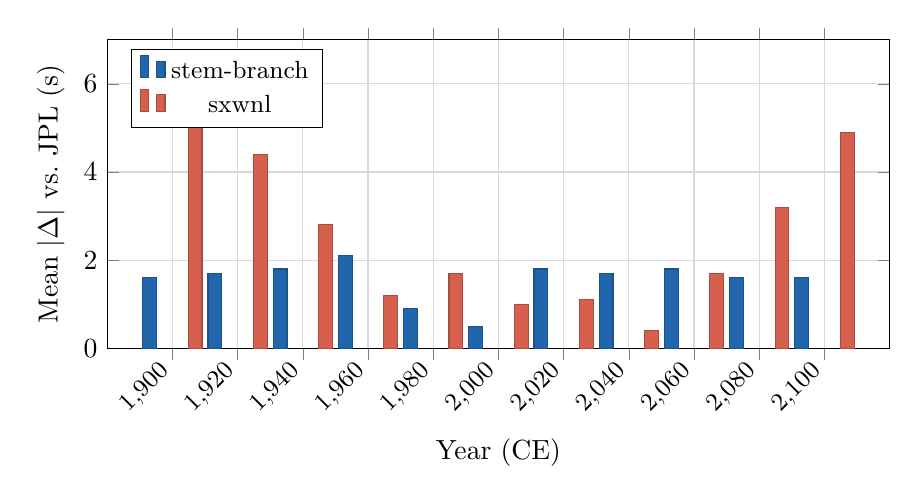
\begin{tikzpicture}
\begin{axis}[
    width=0.95\textwidth,
    height=5.5cm,
    ybar,
    bar width=5pt,
    xlabel={Year (CE)},
    ylabel={Mean $|\Delta|$ vs.\ JPL (s)},
    xmin=1880, xmax=2120,
    ymin=0, ymax=7,
    grid=major,
    grid style={gray!30},
    xtick={1900,1920,1940,1960,1980,2000,2020,2040,2060,2080,2100},
    xticklabel style={rotate=45, anchor=east, font=\small},
    legend pos=north west,
    legend style={font=\small},
]
\addplot[fill=sbblue, draw=sbblue!80!black] coordinates {
    (1896,1.6) (1916,1.7) (1936,1.8) (1956,2.1)
    (1976,0.9) (1996,0.5) (2016,1.8) (2036,1.7)
    (2056,1.8) (2076,1.6) (2096,1.6)
};
\addlegendentry{stem-branch}
\addplot[fill=sxorange, draw=sxorange!80!black] coordinates {
    (1904,5.9) (1924,4.4) (1944,2.8) (1964,1.2)
    (1984,1.7) (2004,1.0) (2024,1.1) (2044,0.4)
    (2064,1.7) (2084,3.2) (2104,4.9)
};
\addlegendentry{sxwnl}
\end{axis}
\end{tikzpicture}
\caption{Head-to-head comparison (1900--2100). sxwnl exhibits a U-shaped curve
minimized near 2040 (close to its DE405 fitting epoch), degrading to 5.9\,s at
1900 and 4.9\,s at 2100. stem-branch maintains $\leq 2.1$\,s throughout.}
\label{fig:sb_vs_sx}
\end{figure*}

\subsection{Percentile Analysis}

\begin{figure}[H]
\centering
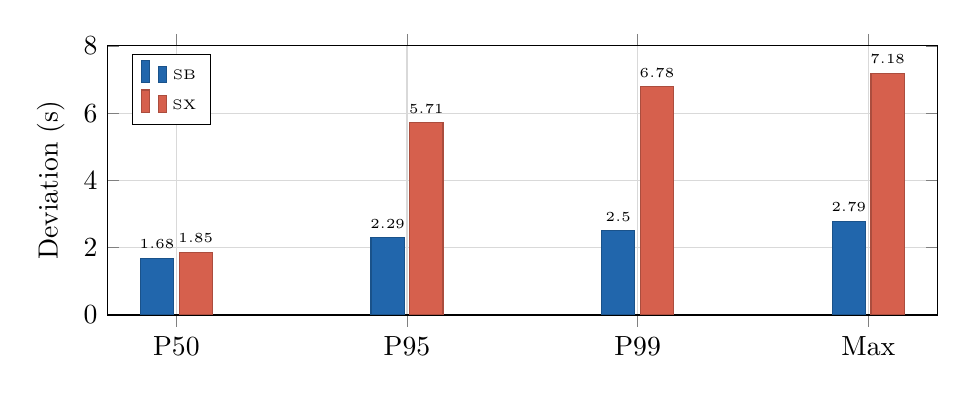
\begin{tikzpicture}
\begin{axis}[
    width=\columnwidth,
    height=5cm,
    ybar,
    bar width=12pt,
    ylabel={Deviation (s)},
    symbolic x coords={P50,P95,P99,Max},
    xtick=data,
    ymin=0, ymax=8,
    grid=major,
    grid style={gray!30},
    legend pos=north west,
    legend style={font=\tiny},
    nodes near coords,
    nodes near coords style={font=\tiny, above},
]
\addplot[fill=sbblue, draw=sbblue!80!black] coordinates {
    (P50,1.68) (P95,2.29) (P99,2.50) (Max,2.79)
};
\addlegendentry{SB}
\addplot[fill=sxorange, draw=sxorange!80!black] coordinates {
    (P50,1.85) (P95,5.71) (P99,6.78) (Max,7.18)
};
\addlegendentry{SX}
\end{axis}
\end{tikzpicture}
\caption{Percentile comparison vs.\ JPL (1900--2100). Medians are comparable,
but tail behavior diverges: stem-branch's P95 is $2.5\times$ lower.}
\label{fig:percentiles}
\end{figure}

\subsection{Deviation Distribution}

Cross-validation between stem-branch and sxwnl covers 4,824 solar terms
(201~years $\times$ 24 terms, 1900--2100). The divergence reflects
differing correction polynomials, not implementation errors.

\begin{figure}[H]
\centering
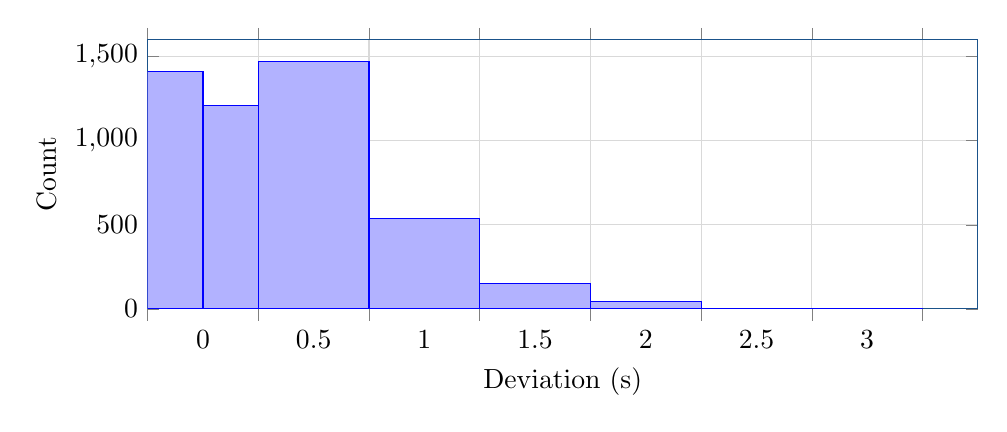
\begin{tikzpicture}
\begin{axis}[
    width=\columnwidth,
    height=5cm,
    ybar interval,
    xlabel={Deviation (s)},
    ylabel={Count},
    xmin=0, xmax=3.75,
    ymin=0, ymax=1600,
    xtick={0,0.5,1.0,1.5,2.0,2.5,3.0,3.5},
    grid=major,
    grid style={gray!30},
    fill=sbblue!60,
    draw=sbblue!80!black,
]
\addplot coordinates {
    (0,1410) (0.25,1209) (0.5,1470) (1.0,540)
    (1.5,149) (2.0,42) (2.5,3) (3.0,1) (3.5,0)
};
\end{axis}
\end{tikzpicture}
\caption{Distribution of SB--SX deviations ($N = 4{,}824$).
54.3\% within 0.5\,s, 84.8\% within 1\,s.}
\label{fig:distribution}
\end{figure}

\subsection{Equinox Amplification}

The deviation by solar term shows double peaks at the equinoxes
($\lambda_\odot = 0\degree$, $180\degree$). This pattern reflects the
interaction between the differing correction polynomials used by
stem-branch and sxwnl: the polynomial residuals are not uniformly
distributed across ecliptic longitude, and the equinox regions---where
the Sun's ecliptic longitude changes most rapidly in right
ascension---amplify small longitude differences into larger timing
differences.

\begin{figure*}[t]
\centering
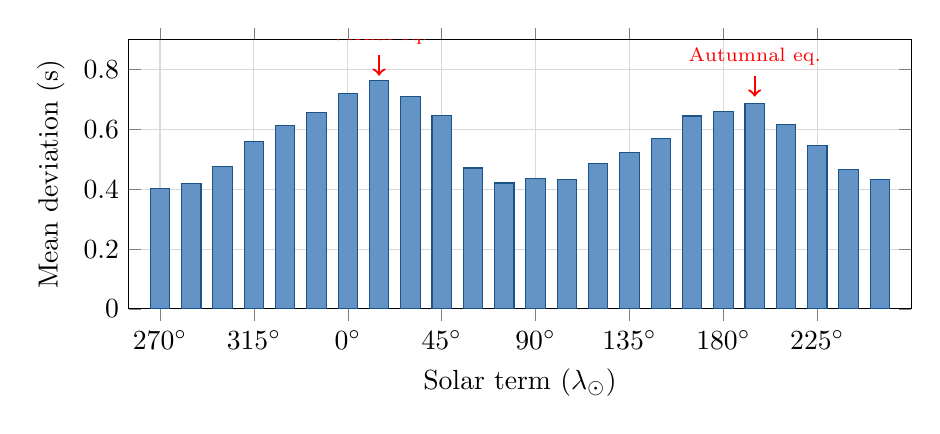
\begin{tikzpicture}
\begin{axis}[
    width=0.95\textwidth,
    height=5cm,
    ybar,
    bar width=7pt,
    xlabel={Solar term ($\lambda_\odot$)},
    ylabel={Mean deviation (s)},
    xmin=-1, xmax=24,
    ymin=0, ymax=0.9,
    xtick={0,3,6,9,12,15,18,21},
    xticklabels={$270\degree$,$315\degree$,$0\degree$,$45\degree$,
                 $90\degree$,$135\degree$,$180\degree$,$225\degree$},
    grid=major,
    grid style={gray!30},
]
\addplot[fill=sbblue!70, draw=sbblue!80!black] coordinates {
    (0,0.404) (1,0.418) (2,0.477) (3,0.559) (4,0.614) (5,0.657)
    (6,0.719) (7,0.765) (8,0.710) (9,0.646) (10,0.471) (11,0.421)
    (12,0.436) (13,0.433) (14,0.486) (15,0.524) (16,0.570) (17,0.645)
    (18,0.661) (19,0.688) (20,0.617) (21,0.545) (22,0.465) (23,0.432)
};
\draw[red, thick, ->] (axis cs:7,0.85) -- (axis cs:7,0.78)
    node[above, pos=0, font=\scriptsize, red] {Vernal eq.};
\draw[red, thick, ->] (axis cs:19,0.78) -- (axis cs:19,0.71)
    node[above, pos=0, font=\scriptsize, red] {Autumnal eq.};
\end{axis}
\end{tikzpicture}
\caption{Mean SB--SX deviation by solar term. Peaks near the equinoxes
and valleys near the solstices reflect the non-uniform distribution of
correction polynomial residuals across ecliptic longitude.}
\label{fig:byterm}
\end{figure*}

\subsection{Four Pillar Agreement}

\begin{table}[H]
\centering
\caption{Pillar cross-validation: SB vs.\ sxwnl}
\label{tab:pillars}
\footnotesize
\begin{tabular}{lccc}
\toprule
\textbf{Pillar} & \textbf{$N$} & \textbf{Range} & \textbf{Agree} \\
\midrule
\zh{日柱} (Day) & 5,683 & 1583--2500 & 100\% \\
\zh{年柱} (Year) & 2,412 & 1900--2100 & 100\% \\
\zh{月柱} (Month) & 2,412 & 1900--2100 & 100\% \\
\bottomrule
\end{tabular}
\end{table}

% =============================================================================

% =============================================================================
\section{Discussion}
\label{sec:discussion}

\subsection{The Computational Error Budget}

For modern-epoch charts (post-1900), the dominant errors are:

\begin{enumerate}
  \item True solar time correction: 0--176~min (avoidable).
  \item Equation of time: $\pm 16$~min (must compute).
  \item DST: 0 or 60~min (requires birth location data).
  \item Day boundary: 0--60+~min (methodological choice).
  \item \zh{閏月} assignment: 0 or catastrophic (rare but severe; see 2033).
  \item Solar terms: $\sim 1$--$3$~s (negligible with proper ephemeris).
  \item $\Delta T$: $< 1$~s (negligible for modern dates).
\end{enumerate}

The irony persists: most software focuses on items~6--7 while ignoring
items~1--5.

\subsection{Historical Chart Reconstruction}

Before $\sim$1600~CE, $\Delta T$ uncertainty exceeds pillar transition
widths for $\sim 0.2$--$0.3$\% of birth times, making the correct pillar
\emph{unknowable} from computation alone. This applies equally to all five
systems: \zh{八字} pillars, \zh{奇門遁甲} formations, \zh{紫微斗數}
palace assignments, \zh{大六壬} \zh{月將} determinations, and
\zh{七政四餘} mansion placements.

% =============================================================================

% =============================================================================
\section{Conclusion}
\label{sec:conclusion}

We have identified seven categories of computational error affecting five
Chinese metaphysical systems and demonstrated that the most impactful
errors are the most neglected. The \texttt{stem-branch} library achieves
$1.05 \pm 0.97$~s (mean $\pm$ P50) solar term accuracy against JPL~DE441
across 2,284~years, with 100\% pillar agreement across 10,507
cross-validation tests.

The expanded analysis reveals that all five systems---\zh{八字},
\zh{奇門遁甲}, \zh{紫微斗數}, \zh{大六壬}, and \zh{七政四餘}---share a
unified dependency on the same astronomical computational pipeline,
ranging from purely solar (\zh{八字}) through solar-lunar (\zh{紫微斗數},
\zh{大六壬}) to fully planetary (\zh{七政四餘}). The case of
\zh{七政四餘} is particularly instructive: a system that was marginalized
for centuries precisely because of accumulated ephemeris errors has been
revitalized by modern planetary computation (Swiss Ephemeris/JPL~DE431),
achieving positional accuracy roughly ten million times better than its
traditional tables. The \zh{拆補法}--\zh{置閏法} controversy in
\zh{奇門遁甲} and the \zh{閏月} problem in \zh{紫微斗數} are
structurally analogous: both are intercalation mechanisms reconciling
incommensurate cycles, and both require precise solar term timing as
their foundation.

The cross-civilizational analysis of reference meridians
(Section~\ref{sec:meridians}) demonstrates that the \zh{洛陽} longitude
debate is not a parochial anomaly but an instance of a universal pattern:
every major astronomical tradition---Chinese, Indian, Greek, Islamic---anchored
its calculations to a ``center of the world'' that was simultaneously a
sacred site and a practical coordinate origin. The Indian
\textit{deshantara} correction from Ujjain is structurally identical to the
true solar time correction in Eq.~\eqref{eq:tst}. The 1884 Greenwich
standardization resolved the Western version of this problem politically;
the Chinese version remains unresolved for metaphysical computation, where
the choice among Luoyang ($112.45\degree$E), Beijing ($116.4\degree$E),
and the UTC+8 standard ($120\degree$E) produces differences of up to
30~minutes---sufficient to affect 4.2\% of birth charts.

Software developers implementing these systems should prioritize:
(1)~correct \zh{立春} boundaries,
(2)~true solar time with explicit longitude and Equation of Time corrections,
(3)~DST handling via embedded IANA transition data,
(4)~explicit day boundary convention,
(5)~full planetary theory with nutation and aberration, and
(6)~documentation of the reference longitude assumed.
For \zh{紫微斗數} and \zh{大六壬}, accurate lunar ephemeris is equally
critical; for \zh{七政四餘}, accurate planetary ephemeris for all seven
classical bodies is the sine qua non of the entire system.

Whether any of these systems produces valid predictions about human
affairs is a question this paper does not address.  What it
demonstrates is that the astronomical computations underlying them
can be made correct---and that most current implementations fail to
do so.

% =============================================================================
\section*{Data Availability}

All scripts, fixtures, and test suites are available at
\url{https://github.com/h4x0r/stem-branch}. Reproduce via:

{\small
\begin{verbatim}
node scripts/jpl-comparison.mjs
node scripts/jpl-3way-solar-terms.mjs
npx vitest run tests/cross-validation
\end{verbatim}
}

\section*{Acknowledgements}

The author acknowledges \zh{許劍偉} (Xu Jianwei) and sxwnl for the
cross-validation reference, JPL Horizons for ground truth data, and the
foundational work of Stephenson, Morrison, Hohenkerk ($\Delta T$) and
Yuk Tung Liu (\zh{廖育棟}, Chinese calendar methodology).

% =============================================================================

% =============================================================================
\begin{sloppypar}
\begin{thebibliography}{99}

\bibitem{stephenson2016}
F.~R. Stephenson, L.~V. Morrison, and C.~Y. Hohenkerk,
``Measurement of the Earth's rotation: 720~BC to AD~2015,''
\textit{Proc. R. Soc. A}, vol.~472, no.~2196, 2016.

\bibitem{stephenson1986}
F.~R. Stephenson and M.~A. Houlden,
\textit{Atlas of Historical Eclipse Maps: East Asia, 1500~BC--AD~1900}.
Cambridge Univ. Press, 1986.

\bibitem{stephenson2018}
F.~R. Stephenson, L.~V. Morrison, and C.~Y. Hohenkerk,
``The provenance of early Chinese records of large solar eclipses,''
\textit{J. Hist. Astron.}, vol.~49, no.~4, pp.~447--477, 2018.

\bibitem{bretagnon1988}
P.~Bretagnon and G.~Francou,
``Planetary theories in rectangular and spherical variables: VSOP87,''
\textit{Astron. Astrophys.}, vol.~202, pp.~309--315, 1988.

\bibitem{meeus1998}
J.~Meeus,
\textit{Astronomical Algorithms}, 2nd ed.
Willmann-Bell, 1998.

\bibitem{iau2000b}
D.~D. McCarthy and B.~J. Luzum,
``An abridged model of the precession-nutation of the celestial pole,''
\textit{Celest. Mech. Dyn. Astron.}, vol.~85, no.~1, pp.~37--49, 2003.

\bibitem{ronvondrak1986}
C.~Ron and J.~Vondr\'{a}k,
``Expansion of annual aberration into trigonometric series,''
\textit{Bull. Astron. Inst. Czechoslov.}, vol.~37, pp.~96--103, 1986.

\bibitem{aslaksen2010}
H.~Aslaksen,
``The mathematics of the Chinese calendar,''
NUS, Tech. Rep., 2010.

\bibitem{aslaksen_fake}
H.~Aslaksen,
``Fake leap months in the Chinese calendar: From the Jesuits to 2033,''
\textit{Academia.edu preprint}, 2017.

\bibitem{sxwnl_github}
\zh{許劍偉} (Xu Jianwei),
``\zh{壽星天文曆} 5.10,''
GitHub, 2024.

\bibitem{jpl_horizons}
JPL, ``Horizons System,'' NASA/JPL Solar System Dynamics.
\url{https://ssd.jpl.nasa.gov/horizons/}

\bibitem{jpl_de441}
R.~S. Park et al.,
``The JPL Planetary and Lunar Ephemerides DE440 and DE441,''
\textit{Astron. J.}, vol.~161, no.~3, p.~105, 2021.

\bibitem{nasa_deltaT_uncertainty}
F.~Espenak, ``Uncertainty in $\Delta T$,'' NASA Eclipse Web Site, 2009.

\bibitem{spencer1971}
J.~W. Spencer, ``Fourier series representation of the position of the Sun,''
\textit{Search}, vol.~2, no.~5, p.~172, 1971.

\bibitem{ytliu_solarterms}
Y.~T. Liu, ``24 Solar Terms,''
\url{https://ytliu0.github.io/ChineseCalendar/solarTerms.html}

\bibitem{ytliu_computation}
Y.~T. Liu, ``Calendar Calculation,''
\url{https://ytliu0.github.io/ChineseCalendar/computation.html}

\bibitem{ytliu_rules}
Y.~T. Liu, ``Rules for the Chinese Calendar,''
\url{https://ytliu0.github.io/ChineseCalendar/rules.html}

\bibitem{ytliu_sunmoon}
Y.~T. Liu, ``Calculation of Moon Phases and 24 Solar Terms,''
\url{https://ytliu0.github.io/ChineseCalendar/docs/sunMoon.pdf}

\bibitem{eddy1976}
J.~A. Eddy, ``The Maunder Minimum,''
\textit{Science}, vol.~192, pp.~1189--1202, 1976.

\bibitem{hayakawa2017}
H.~Hayakawa et al.,
``Records of sunspot and aurora candidates in Chinese official histories,
1261--1644,''
\textit{Publ. Astron. Soc. Jpn.}, vol.~69, no.~4, 2017.

\bibitem{hayakawa2022}
H.~Hayakawa et al.,
``Rediscovery of 23 historical records of naked-eye sunspot observations
in AD~1618,''
\textit{Sol. Phys.}, vol.~297, no.~9, 2022.

\bibitem{zhukz1973}
\zh{竺可楨},
``\zh{中國近五千年來氣候變遷的初步研究},''
\textit{\zh{考古學報}}, no.~1, pp.~15--38, 1973.

\bibitem{eclipse709bce_2025}
M.~Soma, K.~Tanikawa, et al.,
``2,700-year old eclipse mystery,''
\textit{EurekAlert!}, 2025.

\bibitem{wikipedia_fourpillars}
``Four Pillars of Destiny,'' Wikipedia.

\bibitem{wikipedia_2033}
``\zh{2033年問題},'' \zh{維基百科}.

\bibitem{gbstandard2017}
GB/T~33661-2017, ``\zh{農曆的編算和頒行},'' 2017.

\bibitem{unesco2016}
UNESCO, ``The Twenty-Four Solar Terms,'' ICH Decision 11.COM 10.b.14, 2016.

\bibitem{yanbo_diaosou}
``\zh{煙波釣叟賦},'' authorship disputed (traditionally attributed to
\zh{趙普}, Song dynasty chancellor, 922--992~CE; modern scholarship
considers this attribution spurious). The text likely originates from the
Northern Song or Yuan period. Canonical verse encoding the \zh{置閏法}
method of \zh{奇門遁甲}.

\bibitem{dunjia_fuying}
``\zh{遁甲符應經},'' compiled during the Jingyou era (\zh{景祐},
1034--1038~CE), Song dynasty. First documented source for the
\zh{拆補法} method of \zh{奇門遁甲}.

\bibitem{zwds_quanshu}
\zh{羅洪先} (attr.), ``\zh{紫微斗數全書},'' Ming dynasty. One of the two
canonical texts of \zh{紫微斗數}; contains the \zh{安身命例} prescribing
Approach~2 for \zh{閏月}.

\bibitem{zwds_quanji}
``\zh{紫微斗數全集},'' Ming dynasty. The second canonical text; explicitly
rejects solar-term-based month determination.

\bibitem{doushu_xuanwei}
``\zh{斗數宣微},'' date uncertain. Prescribes the 15th-day split method
(Approach~3) for \zh{閏月} in \zh{紫微斗數}.

\bibitem{xingli_kaoyuan}
\zh{梅文鼎} et~al., ``\zh{星歷考原},'' Qing dynasty, 1713. Cites
\zh{汲冢周書} in support of the 15th-day split for intercalary months.

\bibitem{jingyou_liuren}
\zh{楊惟德}, ``\zh{景祐六壬神定經},'' Song dynasty, 1034~CE. Redefined
\zh{月將} determination using the \zh{日躔法} (sidereal lodge method).

\bibitem{mengxi_bitan}
\zh{沈括}, ``\zh{夢溪筆談},'' c.~1088. Identified the precession-induced
divergence between \zh{合神法} and \zh{日躔法} in \zh{大六壬}.

\bibitem{eliade1958}
M.~Eliade,
\textit{Patterns in Comparative Religion}.
Sheed \& Ward, 1958.

\bibitem{needham1959}
J.~Needham,
\textit{Science and Civilisation in China}, vol.~3:
\textit{Mathematics and the Sciences of the Heavens and the Earth}.
Cambridge Univ. Press, 1959.

\bibitem{cullen1996}
C.~Cullen,
\textit{Astronomy and Mathematics in Ancient China: The Zhou Bi Suan Jing}.
Cambridge Univ. Press, 1996.

\bibitem{sivin2009}
N.~Sivin,
\textit{Granting the Seasons: The Chinese Astronomical Reform of 1280}.
Springer, 2009.

\bibitem{udias1994}
A.~Ud\'{\i}as,
``Jesuit Astronomers in Beijing 1601--1805,''
\textit{Q. J. R. Astron. Soc.}, vol.~35, pp.~463--478, 1994.

\bibitem{burgess1860}
E.~Burgess (trans.),
\textit{The Surya Siddhanta: A Text-Book of Hindu Astronomy}.
American Oriental Society, 1860. Repr.\ Motilal Banarsidass, 2000.

\bibitem{shukla1976}
K.~S.~Shukla and K.~V.~Sarma,
\textit{Aryabhatiya of Aryabhata}.
Indian National Science Academy, 1976.

\bibitem{plofker2009}
K.~Plofker,
\textit{Mathematics in India}.
Princeton Univ. Press, 2009.

\bibitem{berggren2000}
J.~L. Berggren and A.~Jones,
\textit{Ptolemy's Geography: An Annotated Translation of the Theoretical
Chapters}.
Princeton Univ. Press, 2000.

\bibitem{kennedy1956}
E.~S. Kennedy,
``A survey of Islamic astronomical tables,''
\textit{Trans. Am. Philos. Soc.}, vol.~46, no.~2, pp.~123--177, 1956.

\bibitem{pingree1970}
D.~Pingree,
``The fragments of the works of al-Fazari,''
\textit{J. Near East. Stud.}, vol.~29, no.~2, pp.~103--123, 1970.

\bibitem{sayili1960}
A.~Say{\i}l{\i},
\textit{The Observatory in Islam}.
Turkish Historical Society, 1960. Repr.\ Arno Press, 1981.

\bibitem{sobel1995}
D.~Sobel,
\textit{Longitude: The True Story of a Lone Genius Who Solved the Greatest
Scientific Problem of His Time}.
Walker \& Co., 1995.

\bibitem{howse1997}
D.~Howse,
\textit{Greenwich Time and the Longitude}.
Philip Wilson, 1997.

\bibitem{patrick1974}
J.~Patrick,
``Midwinter sunrise at Newgrange,''
\textit{Nature}, vol.~249, pp.~517--519, 1974.

\bibitem{aveni2001}
A.~F. Aveni,
\textit{Skywatchers: A Revised and Updated Version of Skywatchers of Ancient
Mexico}.
Univ. of Texas Press, 2001.

\bibitem{harley1987}
J.~B. Harley and D.~Woodward (eds.),
\textit{The History of Cartography}, vol.~1:
\textit{Cartography in Prehistoric, Ancient, and Medieval Europe and the
Mediterranean}.
Univ. of Chicago Press, 1987.

\bibitem{aylward2007}
T.~F. Aylward,
\textit{The Imperial Guide to Feng Shui and Chinese Astrology: The Original
Chinese Text with Translation}.
Watkins, London, 2007.

\bibitem{pmo_lte440}
Purple Mountain Observatory,
``LTE440: A Lunar Time Ephemeris,''
\textit{Astronomy \& Astrophysics}, 2025.

\bibitem{huang_tungshu}
\zh{黃一農}, research on Taiwanese \zh{通勝} traditions and the
\zh{繼成堂} lineage.

\bibitem{choi_intangible}
Guangdong Provincial Government,
``\zh{蔡真步堂通勝} recognized as provincial-level intangible cultural
heritage,'' 2013.

\bibitem{xieji_bianfang}
\zh{允祿} et~al. (comp.),
``\zh{欽定協紀辨方書},'' 36~juan, Qing dynasty, 1739.
Partial English translation: \cite{aylward2007}.

\bibitem{niu_weixing_1995}
\zh{牛維星}, ``An Inquiry into the Astronomical Meaning of Rahu and Ketu,''
\textit{Chinese Astronomy and Astrophysics}, vol.~19, pp.~259--270, 1995.

\bibitem{kotyk_2017}
J.~Kotyk, ``Buddhist Astrology and Astral Magic in the Tang Dynasty,''
Ph.D. dissertation, Leiden University, 2017.

\bibitem{kotyk_2018}
J.~Kotyk, ``The Sinicization of Indo-Iranian Astrology in Medieval China,''
\textit{Sino-Platonic Papers}, no.~282, 2018.

\bibitem{ho_peng_yoke_2003}
Ho Peng Yoke, \textit{Chinese Mathematical Astrology: Reaching Out for the
Stars}, Needham Research Institute Series, RoutledgeCurzon, London, 2003.

\bibitem{lu_schall_2020}
L\"u, ``When Missionary Astronomy Encountered Chinese Astrology: Johann Adam
Schall von Bell and Chinese Calendar Reform,'' \textit{Physics in
Perspective}, vol.~22, pp.~110--130, 2020.

\bibitem{swiss_ephemeris}
D.~Koch and A.~Treindl, ``Swiss Ephemeris,'' Astrodienst AG,
Zollikon/Zurich. Based on NASA JPL DE431.

\bibitem{taisui_origin}
\zh{盧央}, ``\zh{從「歲星」到「太歲」},''
\textit{Journal of Chinese Studies}, 2013.
See also: ``\zh{太歲},'' \zh{維基百科}.

\bibitem{smith_2011}
A.~Smith, ``The Chinese Sexagenary Cycle and the Ritual Origins of the
Calendar,'' in \textit{Calendars and Years II: Astronomy and Time in the
Ancient and Medieval World}, Oxbow Books, 2011.

\bibitem{china_timezone}
IANA Time Zone Database (\texttt{tzdata}), zone \texttt{Asia/Shanghai}
and \texttt{Asia/Urumqi}.
\url{https://www.iana.org/time-zones}

\bibitem{china_timezones_1918}
``Time in China,'' Wikipedia.
\url{https://en.wikipedia.org/wiki/Time_in_China}
See also: IANA \texttt{tzdata} file \texttt{asia}, which documents the
1918 five-zone proposal and the 1949 unification.

\bibitem{qiyao_rangzai}
``\zh{七曜攘災決},'' 806~CE. Taisho Buddhist canon T~1308. Preserved only
in Japan; brought by monk Sh\=uei (\zh{宗叡}) in 865~CE.

\bibitem{zhang_zhichun}
\zh{張志春}, ``\zh{神奇之門},'' (\textit{The Miraculous Door}).
Influential modern text advocating the \zh{拆補法} method in
\zh{奇門遁甲}.

\bibitem{scmp_choi_obituary}
``Hong Kong feng shui master Choi Pak-lai dies aged 96,''
\textit{South China Morning Post}, July 2018.
\url{https://www.scmp.com/news/hong-kong/community/article/2156992/}

\bibitem{initium_choi_2019}
``\zh{蔡興華}: \zh{通勝編纂四代傳承},'' \textit{Initium Media}, February 2019.
\url{https://theinitium.com/article/20190202-culture-hongkong-traditional-calendar}

\bibitem{hko_calendar_history}
Hong Kong Observatory, ``A Brief History about the Authoritative
Organizations for Compiling Calendar in China.''
HKO Education Series.
\url{https://www.hko.gov.hk/en/education/astronomy-and-time/}

\bibitem{huang_yilong_planets}
\zh{黃一農}, studies on Chinese planetary calculation accuracy
and the \zh{歲星紀年} system, National Tsing Hua University.

\bibitem{xing_yunlu}
\zh{邢雲路} (1573--1620), ``\zh{古今律曆考},'' Ming dynasty. Advocated
midnight (\zh{夜半}) as the start of \zh{子時}.

% ── 共盤問題 references ──────────────────────────────────────

\bibitem{smith_fortune_2019}
R.~J. Smith, \textit{Fortune-tellers and Philosophers: Divination in
Traditional Chinese Society}, Routledge, 2019 (orig.\ 1991).
ISBN 978-0-367-15980-1.

\bibitem{raphals_2003}
L.~Raphals, ``Fate, Fortune, Chance, and Luck in Chinese and Greek:
A Comparative Study,'' \textit{Philosophy East and West}, vol.~53, no.~4,
pp.~537--574, 2003.
\url{https://www.jstor.org/stable/1400052}

\bibitem{geng_li_2019}
Geng Li, \textit{Fate Calculation Experts: The Practice and Authority of
Chinese Fortune-telling}, Berghahn Books, 2019.
ISBN 978-1-78533-994-3.

\bibitem{chao_weipang_1946}
Chao Wei-pang, ``The Chinese Science of Fate-Calculation,''
\textit{Folklore Studies}, vol.~5, pp.~1--40, 1946.
\url{https://www.jstor.org/stable/1177422}

\bibitem{sanming_tonghui}
\zh{萬民英} (Wan Minying), ``\zh{三命通會},'' Ming dynasty, c.~1550.
12~juan; the most comprehensive classical compilation of fate-calculation
methods. Available at Chinese Text Project:
\url{https://ctext.org/wiki.pl?if=en&res=758991}

\bibitem{ditian_sui}
\zh{京圖} (Jing Tu), attrib., ``\zh{滴天髓},'' Song dynasty (attrib.);
Qing dynasty commentary by \zh{任鐵樵} (Ren Tieqiao), c.~1820--1850.

\bibitem{ziping_zhenquan}
\zh{沈孝瞻} (Shen Xiaozhan), ``\zh{子平真詮},'' Qing dynasty.
First published 1779; modern standard ed.\ by
\zh{方重審} and \zh{徐樂吾}, 1936.

\bibitem{qiongtong_baojian}
\zh{余春台} (Yu Chuntai), ``\zh{窮通寶鑑},'' Qing dynasty.
Seasonal adjustment (\zh{調候}) school of fate calculation.

% ── DST references ───────────────────────────────────────────

\bibitem{iana_tzdata_asia}
IANA Time Zone Database (\texttt{tzdata}), file \texttt{asia}.
Primary source for all East Asian DST transition dates and rules.
Commentary by Paul Eggert, Arthur~D. Olson, et~al.
\url{https://data.iana.org/time-zones/tz-link.html}

\bibitem{hko_summertime}
Hong Kong Observatory, ``Summer-time Arrangements in Hong Kong.''
\url{https://www.hko.gov.hk/en/gts/time/stehistory.htm}

\bibitem{prc_dst_regulation}
State Council of the PRC, ``\zh{國務院關於在全國範圍內實行夏時制的通知}''
(``Notice on Implementing Summer Time Nationwide''),
4~April~1986. Effective 1986--1991.

\bibitem{japan_dst_abolition}
``Daylight saving time in Japan,'' in \textit{Summer Time}, Wikipedia.
53\% opposed vs.\ 30\% in favor per 1951 government survey;
Diet abolished DST in October 1951 after San Francisco Peace Treaty.
\url{https://en.wikipedia.org/wiki/Daylight_saving_time_in_Japan}

\bibitem{korea_tz_history}
``Time in South Korea,'' Wikipedia.
Documents the UTC$+$8:30 $\leftrightarrow$ UTC$+$9 oscillations
(1908--1912--1954--1961) and 1987--1988 Seoul Olympics DST.
\url{https://en.wikipedia.org/wiki/Time_in_South_Korea}
See also: IANA \texttt{tzdata} file \texttt{asia}, Rule ROK.

\bibitem{wetoasthk_dst}
WeToastHK, ``\zh{香港夏令時間的歷史}'' (``History of Hong Kong
Summer Time''), 2017.
Detailed legislative narrative citing original Legislative Council
documents, South China Morning Post reports, and Governor's proclamations.
Provides transition times (e.g.\ 1946: 17:00) not available from HKO,
clarifies that 1942--1945 was JST imposition (not DST), and documents
the 1945 November~18 standard-time restoration.
\url{https://www.wetoasthk.com/1010-2/}

\bibitem{dst_east_asia_research}
\texttt{stem-branch} project, ``East Asian DST History ---
Comprehensive Research,'' \texttt{docs/research/east-asia-dst-history.md}.
Complete IANA rule definitions for 7~regions: PRC, Taiwan, Hong Kong,
Macau, Japan, South Korea, Mongolia.
\url{https://github.com/h4x0r/stem-branch}

% ── Methodological references ────────────────────────────────

\bibitem{xieji_bianfangshu}
\zh{允祿} (Prince Yunlu), \zh{梅瑴成} (Mei Juecheng),
\zh{何國宗} (He Guozong), et~al., ``\zh{協紀辯方書}''
(\textit{Treatise on the Harmonization of Times and Distinction of
Directions}), 1739. Imperially commissioned compendium that
systematically audited and purged fabricated calendar spirits and
divinatory heuristics.

\bibitem{aylward_imperial_guide}
Thomas~F. Aylward, \textit{The Imperial Guide to Feng Shui \&
Chinese Astrology: The Only Authentic Translation from the Original
Chinese}, London: Watkins, 2007. Partial English translation of the
\zh{協紀辯方書}.

\bibitem{bruun_fengshui}
Ole Bruun, \textit{Fengshui in China: Geomantic Divination Between
State Orthodoxy and Popular Religion}, Honolulu: University of
Hawai'i Press, 2003; also \textit{An Introduction to Feng Shui},
Cambridge University Press, 2008.

\bibitem{fernandez_beanato_2021}
Dami\'{a}n Fernandez-Beanato, ``Feng Shui and the Demarcation
Project,'' \textit{Science \& Education}, vol.~30, pp.~1333--1351,
2021. Analyzes the ``karmic stratagem'' that renders \zh{風水}
unfalsifiable through surplus interpretive degrees of freedom.

\bibitem{lackner_zhao_2022}
Michael Lackner and Zhao~Lu, eds., \textit{Handbook of Divination
and Prognostication in China}, Leiden: Brill, 2022. Comprehensive
scholarly reference; discusses \zh{鐵板神數} attribution and
dating.

\bibitem{huangdi_neijing}
\zh{黃帝內經} (\textit{Huangdi Neijing}, ``Inner Canon of the
Yellow Emperor''), compiled Warring States--Han dynasty. Foundational
TCM text establishing the prenatal \zh{元氣}/postnatal \zh{空氣}
framework that underpins the ``first breath'' birth-time convention.

\bibitem{hashimoto_2004}
Masana Hashimoto, ``Units of Time in Ancient China and Japan,''
\textit{Publications of the Astronomical Society of Japan},
vol.~56, no.~5, p.~887, 2004. Documents the evolution of the
\zh{刻} system from 100~\zh{刻}/day (Han) through 96~\zh{刻}/day
(Qing).

% ── Tropical vs sidereal references ─────────────────────────

\bibitem{toomer_almagest}
Ptolemy, \textit{Ptolemy's Almagest}, trans.\ G.~J. Toomer,
Princeton University Press, 1998. Standard scholarly translation;
discusses Hipparchus's precession discovery and the ecliptic
coordinate system.

\bibitem{ptolemy_tetrabiblos}
Ptolemy, \textit{Tetrabiblos}, trans.\ F.~E. Robbins,
Loeb Classical Library, Harvard University Press, 1940.
Book~I.10 establishes the vernal equinox as the zodiacal origin.

\bibitem{pingree_jyotihsastra}
David Pingree, \textit{Jyoti\d{h}\'{s}\={a}stra: Astral and
Mathematical Literature}, vol.~6, fasc.~4 of \textit{A History of
Indian Literature}, ed.\ J.~Gonda, Wiesbaden: Otto Harrassowitz,
1981. Foundational scholarly reference for Indian mathematical
astrology.

\bibitem{sun_kistemaker_1997}
Sun Xiaochun and Jacob Kistemaker, \textit{The Chinese Sky during
the Han: Constellating Stars and Society}, Sinica Leidensia~38,
Leiden: Brill, 1997. Documents the 28~\zh{宿} sidereal mansion
system and Chinese star catalogues.

\bibitem{hockey_bea_2014}
Thomas Hockey, Virginia Trimble, and Thomas~R. Williams, eds.,
\textit{The Biographical Encyclopedia of Astronomers}, 2nd~ed.,
Springer, 2014. Contains entry on \zh{虞喜} (Yu~Xi) and his
independent discovery of precession.

\bibitem{chandra_hari_1998}
K.~Chandra Hari, ``On the Origin of Siderial Zodiac and Astronomy,''
\textit{Indian Journal of History of Science}, vol.~33, no.~4, 1998.
Analyzes the ayanamsa controversy and sidereal zodiac origins.

\bibitem{wang_tingzhi_tanxing}
Wang~Tingzhi (\zh{王亭之}; Tam~Shek-wing, \zh{談錫永}),
\zh{《王亭之談星》} (\textit{Wang Tingzhi Tan Xing}, ``Wang Tingzhi
on Astrology''), Hong Kong, 1990s.  Critical essays on \zh{紫微斗數}
and related divinatory traditions including
\zh{鐵板神數}; Wang was the Zhongzhou School (\zh{中州派}) lineage
holder and later Visiting Professor of Sino-Tibetan Buddhist Studies,
Renmin University of China.

\end{thebibliography}
\end{sloppypar}

\end{document}
